\documentclass[12pt,]{article}
\usepackage{lmodern}
\usepackage{amssymb,amsmath}
\usepackage{ifxetex,ifluatex}
\usepackage{fixltx2e} % provides \textsubscript
\ifnum 0\ifxetex 1\fi\ifluatex 1\fi=0 % if pdftex
  \usepackage[T1]{fontenc}
  \usepackage[utf8]{inputenc}
\else % if luatex or xelatex
  \ifxetex
    \usepackage{mathspec}
  \else
    \usepackage{fontspec}
  \fi
  \defaultfontfeatures{Ligatures=TeX,Scale=MatchLowercase}
\fi
% use upquote if available, for straight quotes in verbatim environments
\IfFileExists{upquote.sty}{\usepackage{upquote}}{}
% use microtype if available
\IfFileExists{microtype.sty}{%
\usepackage{microtype}
\UseMicrotypeSet[protrusion]{basicmath} % disable protrusion for tt fonts
}{}
\usepackage[margin=1in]{geometry}
\usepackage{hyperref}
\hypersetup{unicode=true,
            pdftitle={In the Shadow of Jim Crow},
            pdfauthor={Kevin Morris},
            pdfborder={0 0 0},
            breaklinks=true}
\urlstyle{same}  % don't use monospace font for urls
\usepackage{longtable,booktabs}
\usepackage{graphicx,grffile}
\makeatletter
\def\maxwidth{\ifdim\Gin@nat@width>\linewidth\linewidth\else\Gin@nat@width\fi}
\def\maxheight{\ifdim\Gin@nat@height>\textheight\textheight\else\Gin@nat@height\fi}
\makeatother
% Scale images if necessary, so that they will not overflow the page
% margins by default, and it is still possible to overwrite the defaults
% using explicit options in \includegraphics[width, height, ...]{}
\setkeys{Gin}{width=\maxwidth,height=\maxheight,keepaspectratio}
\IfFileExists{parskip.sty}{%
\usepackage{parskip}
}{% else
\setlength{\parindent}{0pt}
\setlength{\parskip}{6pt plus 2pt minus 1pt}
}
\setlength{\emergencystretch}{3em}  % prevent overfull lines
\providecommand{\tightlist}{%
  \setlength{\itemsep}{0pt}\setlength{\parskip}{0pt}}
\setcounter{secnumdepth}{5}
% Redefines (sub)paragraphs to behave more like sections
\ifx\paragraph\undefined\else
\let\oldparagraph\paragraph
\renewcommand{\paragraph}[1]{\oldparagraph{#1}\mbox{}}
\fi
\ifx\subparagraph\undefined\else
\let\oldsubparagraph\subparagraph
\renewcommand{\subparagraph}[1]{\oldsubparagraph{#1}\mbox{}}
\fi

%%% Use protect on footnotes to avoid problems with footnotes in titles
\let\rmarkdownfootnote\footnote%
\def\footnote{\protect\rmarkdownfootnote}

%%% Change title format to be more compact
\usepackage{titling}

% Create subtitle command for use in maketitle
\providecommand{\subtitle}[1]{
  \posttitle{
    \begin{center}\large#1\end{center}
    }
}

\setlength{\droptitle}{-2em}

  \title{In the Shadow of Jim Crow}
    \pretitle{\vspace{\droptitle}\centering\huge}
  \posttitle{\par}
  \subtitle{Felony Disenfranchisement and New York State}
  \author{Kevin Morris}
    \preauthor{\centering\large\emph}
  \postauthor{\par}
      \predate{\centering\large\emph}
  \postdate{\par}
    \date{October 17, 2019}

\usepackage{booktabs}
\usepackage{longtable}
\usepackage{array}
\usepackage{multirow}
\usepackage{wrapfig}
\usepackage{float}
\usepackage{colortbl}
\usepackage{pdflscape}
\usepackage{tabu}
\usepackage{threeparttable}
\usepackage{threeparttablex}
\usepackage[normalem]{ulem}
\usepackage{makecell}
\usepackage{xcolor}

\usepackage{setspace}\doublespacing
\usepackage{rotating}

\begin{document}
\maketitle

\pagenumbering{gobble}

\tableofcontents
\pagebreak

\pagenumbering{arabic}

\hypertarget{introduction}{%
\section{Introduction}\label{introduction}}

The political history of the United States has been characterized by a general, if nonlinear, trend toward universal suffrage (see, for instance, Keyssar \protect\hyperlink{ref-Keyssar2009}{2009}). At the time of the nation's founding, access to the ballot box was restricted to landed White men; over the following two centuries, the franchise was greatly expanded. Today, voting rights are considered foundational aspects of full citizenship (United Nations General Assembly Resolution 2200 (XXI)). Despite the United State's march toward ever-more-inclusive systems of democracy, however, one large group of American citizens is formally barred from voting: in most of the country citizens convicted of felonies are at least temporarily prohibited from casting ballots in elections (Brennan Center for Justice \protect\hyperlink{ref-bcj_laws}{2018}). Although some states such as Florida and Louisiana have gradually moved to dismantle their systems of felony disenfranchisement, an estimated 4.7 million American citizens remain disenfranchised (Uggen, Larson, and Shannon \protect\hyperlink{ref-sentencing_2016}{2016}).

The disenfranchisement of citizens convicted of felony offenses intersects with the racialized and place-based patterns of policing and incarceration in the United States. Michelle Alexander (\protect\hyperlink{ref-Alexander2012}{2012}) and others have argued that mass incarceration in the post-Civil Rights era has been used to exert control over minority --- and particularly Black --- Americans. In states such as New York, for instance, the over-representation of minorities among the incarcerated is striking: according to data from the New York State Department of Corrections and Community Supervision, 49.5 percent of individuals who were incarcerated in December of 2018 were non-Hispanic Black, although the Census Bureau estimates that just 14.3 percent of the citizen voting age population in the state is non-Hispanic Black.\footnote{Latinos are also over-represented among the incarcerated population, though not as dramatically: Latinos make up 14.1 percent of the citizen voting age population and 22.9 percent of the incarcerated population.} This disparity is due not to any inherent differential propensity to commit crimes among different racial groups, but rather to systems of policing and concentrated poverty. As Gelman, Fagan, and Kiss (\protect\hyperlink{ref-Gelman2007}{2007}) shows, for instance, New York's ``stop-and-frisk'' policy impacted Black and Latino New Yorkers at rates far higher than Whites, even after controlling for neighborhood characteristics and race-specific criminal propensity.

Due to economic and racial segregation, these effects are highly spatially concentrated. Data available from New York City shows that in 2017, 10 of the New York Police Department's 77 precincts were responsible for more than a quarter of all arrests for felony charges. Many scholars have detailed the impact of living in areas with high levels of police activity. Residents of such neighborhoods suffer from worse physical health (Sewell and Jefferson \protect\hyperlink{ref-Sewell2016}{2016}) and are more likely to suffer from anxiety and exhibit symptoms of trauma (Geller et al. \protect\hyperlink{ref-Geller2014}{2014}). The labor markets and social networks in neighborhoods with high levels of policing and incarceration are disrupted (Clear \protect\hyperlink{ref-Clear2008}{2008}), while concentrated policing has also been credited with having a ``chilling effect'' on neighborhoods' willingness to reach out for help to local governments (Lerman and Weaver \protect\hyperlink{ref-Lerman2013}{2013}).

Felony disenfranchisement policies are part of a criminal justice system that disproportionately impacts Black Americans living in certain communities. The effects of disenfranchisement are concentrated in neighborhoods that already suffer from myriad disadvantages thanks to social and economic marginalization. The neighborhood-specific implications of felony disenfranchisement, however, remain largely unstudied. A number of studies have explored the effect of imprisonment and disenfranchisement on later political participation (White \protect\hyperlink{ref-White2019}{2019}; Gerber et al. \protect\hyperlink{ref-Gerber2014}{2014}; Burch \protect\hyperlink{ref-Burch2011}{2011}). Others have looked at the spillover effects of disenfranchisement on eligible Black voters at the state level (Bowers and Preuhs \protect\hyperlink{ref-Bowers2009}{2009}; King and Erickson \protect\hyperlink{ref-King2016}{2016}). With the exception of Burch (\protect\hyperlink{ref-Burch2013}{2013}), however, little attention has been paid to the impact of felony disenfranchisement on political participation at the neighborhood level.

Filling this gap in the literature is of great importance when we consider the spatial concentration of policing networks. If the spillover effects of felony disenfranchisement are widely dispersed, the political consequences are likely minimal. If, however, the effects are both large enough to be detected at a statewide level (as the literature suggests) but also concentrated in a few neighborhoods, disenfranchisement laws likely severely undermine local political representation This lowered participation can disadvantage neighborhoods insofar as they have unique candidate preferences. It could also lower the resources distributed to these neighborhoods, as politicians determine that too few votes can be won through investing in these areas. This is not merely of theoretical concern: research indicates that turnout differentials at the city level have material consequences. As Hajnal (\protect\hyperlink{ref-Hajnal2009}{2009}) tells us: ``low {[}and uneven{]} turnout results in losses in mayoral elections, less equitable racial and ethnic representation on city councils, and spending policies that are less in line with the preferences of racial and ethnic minorities and other disadvantaged groups'' (8).

The rest of this paper is structured as follows: \textbf{Section 2} discusses the historical context of felony disenfranchisement in the United States, and \textbf{Section 3} provides an overview of the scholarship conducted in the field over the past two decades. \textbf{Section 4} provides an in-depth discussion of the insight extant literature provides for the questions discussed in this project. \textbf{Section 5} presents the data sources used throughout the project.

\textbf{Section 6} proposes a new definition of ``lost voters'' in the context of felony disenfranchisement. I define lost voters as individuals who are not only disenfranchised, but are disenfranchised \emph{and} have a history of participating in elections. This serves as a refinement on past work, which considered only which individuals are formally disenfranchised, regardless of whether they had cast a ballot in the past. Using both a matching model and a standard regression specification, I investigate whether neighborhoods with lost voters saw depressed turnout in the 2017 mayoral election relative to other neighborhoods. The disadvantaged state of neighborhoods with high levels of incarceration has been firmly established; if felony disenfranchisement results in lower turnout among eligible voters in these communities, the literature has likely \emph{understated} the degree to which they are impacted by spatially concentrated patterns of criminal justice. A discussion of the results follows.

\textbf{Section 7} turns from the 2017 mayoral election to the 2018 midterm elections. In early 2018, Governor Andrew Cuomo signed Executive Order 181 which restored voting rights to most individuals in the state who were on parole. I employ an instrumental variables approach to test whether rights restoration boosted turnout among formerly incarcerated individuals. I focus specifically on individuals who would have been eligible to cast a ballot even if the executive order had not gone into effect. A discussion of the results follows.

\textbf{Section 8} synthesizes the findings presented in the rest of the paper and provides concluding remarks.

\hypertarget{background-of-felony-disenfranchisement-in-the-united-states}{%
\section{Background of Felony Disenfranchisement in the United States}\label{background-of-felony-disenfranchisement-in-the-united-states}}

In all but two states (Maine and Vermont), felony disenfranchisement laws ensure that American citizens convicted of felony offenses lose the right to vote for at least some period of time. In some states, such as Oregon and Massachusetts, individuals lose that right only for the period in which they are actively incarcerated. In other states, notably Kentucky and Iowa, felony convictions result in lifelong disenfranchisement unless a returned citizen receives an individual pardon from the state government (Brennan Center for Justice \protect\hyperlink{ref-bcj_laws}{2018}). This variation in laws flows directly from language in the Fourteenth Amendment which allows states to revoke individuals' voting rights ``for participation in rebellion, or other crime.'' The definition of ``other crime,'' left so vague in the Constitution, is now generally used by states to disenfranchise citizens for any felony offense. The Supreme Court, in cases such as \emph{Richardson v. Ramirez} (1974), has upheld states' right to do just that. Collectively, these laws disenfranchise as many as 4.7 million American citizens. Of these, the majority are no longer incarcerated, but are living and working in their communities (Uggen, Larson, and Shannon \protect\hyperlink{ref-sentencing_2016}{2016}).\footnote{The figures reported in Uggen, Larson, and Shannon (\protect\hyperlink{ref-sentencing_2016}{2016}) have been adjusted to reflect the impact of Amendment 4 in Florida.}

Any discussion of felony disenfranchisement in the United States must center the role played by race. As Burch (\protect\hyperlink{ref-Burch2010}{2010}) explains, ``If policies restricting the voting rights of offenders disparately affect one racial group or party, it is because such policies were \emph{intended} to'' (4; emphasis in the original). Previous research has established that the presence of non-White potential voters is associated with the implementation of felony disenfranchisement policies, and that these policies were often adopted during Jim Crow explicitly to reduce the political power of Black Americans (Behrens, Uggen, and Manza \protect\hyperlink{ref-Behrens2003}{2003}). In Florida, to take just one example, felony disenfranchisement was added to the state constitution in 1868. Afterwards, a lawmaker boasted that the amendment had been adopted to prevent the state from being ``niggerized'' (Shofner \protect\hyperlink{ref-florida_1868}{1963}, 374).

The racially unbalanced effects of felony disenfranchisement laws were not confined to the 19th century. Although the Voting Rights Act of 1965 did much to improve access to the ballot box for minorities, it did nothing to undermine the explicitly racialized system of disenfranchisement. Indeed, as the United States has increased the reach of the carceral system in the post-Civil Rights era, the implications of felony disenfranchisement have only grown. As of 2016, more than 10 percent of Black Americans were disenfranchised in 9 states. In Kentucky, the state with the highest level of disenfranchised Black residents, more than one in four Black adults are barred from casting a ballot. Although Black adults made up just 12.1 percent of the voting age population in 2016, they accounted for 36.5 percent of the disenfranchised population (Uggen, Larson, and Shannon \protect\hyperlink{ref-sentencing_2016}{2016}).

Recent data from Florida make the victims of felony disenfranchisement laws especially clear. Prior to January 2019, Floridians convicted of felony offenses were permanently disenfranchised unless they were individually pardoned by a clemency board. In November 2018, voters passed a ballot initiative amending the state constitution to end permanent disenfranchisement. In the first three months after permanent disenfranchisement was ended, 44 percent of formerly incarcerated Floridians who registered to vote were Black --- compared with just 13 percent of the statewide electorate (Morris \protect\hyperlink{ref-Morris2019}{2019}).

\hypertarget{academic-literature-and-felony-disenfranchisement}{%
\section{Academic Literature and Felony Disenfranchisement}\label{academic-literature-and-felony-disenfranchisement}}

In the aftermath of the 2000 presidential election, academic interest in the political implications of felony disenfranchisement was stirred thanks to a paper from Uggen and Manza (\protect\hyperlink{ref-Uggen2002}{2002}). George W. Bush's margin of victory in Florida in 2000 was famously just 537 votes. In their 2002 paper, Uggen and Manza estimate the likely partisan composition of the disenfranchised population with felony convictions in their past. They estimate that if this group had been allowed to vote they would have supported Al Gore by a wide margin. Their enfranchisement, Uggen and Manza argued, would have tipped the presidential contest and resulted in the election of Al Gore. They based their estimates on the voting patterns of eligible individuals who were demographically similar to the disenfranchised population. Though much of the research conducted since their 2002 study has pushed back against some of their key assumptions (namely, that formerly incarcerated individuals turn out at the same rate as demographically-similar individuals who have not been incarcerated), Uggen and Manza convincingly demonstrated that felony disenfranchisement can have material political consequences. In the years after Uggen and Manza published their paper, scholars sought to investigate the relationship between felony disenfranchisement and Black and youth turnout (Miles \protect\hyperlink{ref-Miles2004}{2004}; Hjalmarsson and Lopez \protect\hyperlink{ref-Hjalmarsson2010}{2010}). Some of this research compared states and regions with differing disenfranchisement regimes to estimate these effects (Miles \protect\hyperlink{ref-Miles2004}{2004}; Ochs \protect\hyperlink{ref-Ochs2006}{2006}). Others have used survey data or interviews to construct their estimates (Uggen and Manza \protect\hyperlink{ref-Uggen2004}{2004}; Drucker and Barreras \protect\hyperlink{ref-Drucker2005}{2005}).

In a series of papers between 2009 and 2011, researchers developed methods for directly estimating the turnout of formerly disenfranchised individuals. Haselswerdt (\protect\hyperlink{ref-Haselswerdt2009}{2009}) matched administrative release data and voter registration data from Erie County, NY, to estimate turnout among a small group of formerly incarcerated individuals. Traci Burch (\protect\hyperlink{ref-Burch2010}{2010}, \protect\hyperlink{ref-Burch2011}{2011}) expanded upon this matching methodology to estimate the voting patterns of formerly disenfranchised individuals in a range of states. She used release data from states' Departments of Corrections and their registered voter files to identify formerly incarcerated individuals who went on to register to vote. Using the registered voter files, she was also able to estimate the party affiliation of formerly incarcerated individuals (in states with party registration) and their turnout rates. Her methodology has been used to investigate other questions surrounding the voting patterns of formerly incarcerated individuals under different circumstances and to examine the impact of changes in disenfranchisement policy (e.g.~Meredith and Morse \protect\hyperlink{ref-Meredith2013}{2013}, \protect\hyperlink{ref-Meredith2015}{2015}).

A number of papers have also explored the impact felony disenfranchisement policies have on turnout among non-disenfranchised residents. King and Erickson (\protect\hyperlink{ref-King2016}{2016}), for instance, leverages state-level variation in disenfranchisement laws to estimate the impact that felony disenfranchisement has on turnout among eligible Black Americans. They use data from the 2004 Current Population Survey Voting and Registration Supplement to calculate statewide turnout rates by race, and include estimates of the share of Black citizens who are disenfranchised in each state from Manza and Uggen (\protect\hyperlink{ref-locked_out}{2006}) to explore the impact of these policies on eligible voters. They conclude that disenfranchisement has large spillover effects for Black voters: where more Black residents are disenfranchised, eligible Black voters are less likely to cast a ballot. These findings are in line with other research that has explored whether the effects of disenfranchisement extend beyond those whose voting rights are directly suspended (Bowers and Preuhs \protect\hyperlink{ref-Bowers2009}{2009}; Ochs \protect\hyperlink{ref-Ochs2006}{2006}). As Bowers and Preuhs (\protect\hyperlink{ref-Bowers2009}{2009}) sums up: ``{[}I{]}t is not solely the direct vote of ex-felons that is denied through these laws. {[}Felony disenfranchisement{]} impacts the political power of communities that extends beyond felons' collateral penalty'' (724).

Although scholars have established that felony disenfranchisement decreases turnout among Black voters at the \emph{state} level, relatively little research has been done on how felony disenfranchisement operates at the sub-state level. Though we know that Black voters are generally less likely to cast a ballot when they live in a state with strict disenfranchisement laws, little work has been done exploring the impact these laws might have at the local level. Burch (\protect\hyperlink{ref-Burch2013}{2013}) is an exception to this. Burch explores the depressive effect of disenfranchisement laws at the local level in North Carolina by examining Census block group level turnout and zip code level involvement with the criminal justice system, determining that ``at high concentrations, imprisonment and community supervision have an unequivocally demobilizing effect of neighborhoods'' (185). This project seeks to expand on her work by replicating her findings in New York City; by using a different estimation technique; and by using a different definition of ``lost voters.''

\hypertarget{what-this-paper-examines}{%
\section{What This Paper Examines}\label{what-this-paper-examines}}

This paper begins by exploring the effect of felony disenfranchisement on neighborhood turnout in the New York City mayoral election of 2017 using individual-level administrative data. Policing and incarceration patterns have historically targeted communities of color, damaging the social fabric of these neighborhoods (e.g.~Sewell and Jefferson \protect\hyperlink{ref-Sewell2016}{2016}; Clear \protect\hyperlink{ref-Clear2008}{2008}; Lerman and Weaver \protect\hyperlink{ref-Lerman2013}{2013}). It is possible, however, that these effects run deeper than the direct focus on policing and incarceration has acknowledged. We know that felony disenfranchisement systematically removes individuals from certain neighborhoods, but it is not clear that enough would-be voters are removed relative to the electorate to meaningfully distort neighborhood representation. To the extent that felony disenfranchisement has a spatially-concentrated depressive effect on eligible voters, it is possible that these policies are powerful enough to materially reduce the representation of certain parts of the city.

I begin by offering a refinement of our understanding of who lost voters are. Previous studies exploring the relationship between felony disenfranchisement and spillover effects have not adequately accounted for the fact that many of the disenfranchised are low-propensity voters to begin with. In this analysis, I use administrative data to identify neighborhoods where individuals with a \emph{demonstrated history} of participation are disenfranchised. By matching ``treated'' neighborhoods (neighborhoods with lost voters) to ``untreated'' neighborhoods, I estimate the causal effect of felony disenfranchisement on neighborhood turnout.

After examining the effect of felony disenfranchisement on voter turnout at the neighborhood level, I consider the efficacy of a program intended to undo one piece of the felony disenfranchisement apparatus. In April 2018, Governor Andrew Cuomo signed Executive Order 181 which restored voting rights to New Yorkers on parole.\footnote{Prior to Executive Order 181, residents convicted of felonies in prison and on parole were barred from voting, while individuals sentenced to probation did not have their voting rights revoked. Today, only those currently in prison for felony offenses are disenfranchised.} Parole officers were required to provide registration forms to the parolees under their supervision and inform them of their voting rights. In theory, such a policy could increase turnout and registration for parolees. To test whether the policy was successful, I use administrative data to explore whether turnout rates in the 2018 midterm elections among individuals discharged from parole were impacted by the implementation of Executive Order 181.

The first part of this project seeks to refine how we think about felony disenfranchisement in the United States. Rather than think about it purely through the prism of those directly impacted (residents who are actively disenfranchised) or through a prism of race (by examining the impact of disenfranchisement on Black turnout at the state level), I seek to introduce the importance of physical space into the conversation. This will allow us to both better understand the mechanisms through which the depressive effects operate and also to understand more deeply where these effects are concentrated. Of course, understanding the impact of felony disenfranchisement is not enough: we must also test whether our efforts to undo its legacy are effective. The second part of this project seeks to do just that.

\hypertarget{framing-for-turnout-effects}{%
\subsection*{Framing for Turnout Effects}\label{framing-for-turnout-effects}}
\addcontentsline{toc}{subsection}{Framing for Turnout Effects}

Despite over-incarceration in some neighborhoods, the number of incarcerated individuals is relatively low compared to the number of voters. In New York, for instance, 46,232 individuals were imprisoned in New York State in early 2019, compared with 11.6 million actively registered voters. Despite the low share of residents who are directly disenfranchised, there is reason to believe the policy impacts more individuals than just those imprisoned. As discussed above, previous research has demonstrated that felony disenfranchisement reduces turnout even among Black voters whose rights are not suspended This research has found, in particular, that eligible Black voters are less likely to cast a ballot in states where felony disenfranchisement policies are harsher, an effect often referred to as \emph{de facto} disenfranchisement.

Though previous studies have focused largely on the state-level spillover effects of felony disenfranchisement, there is reason to believe that this \emph{de facto} disenfranchisement is concentrated within the neighborhoods home to formally disenfranchised residents. Burch (\protect\hyperlink{ref-Burch2013}{2013}), for instance, demonstrates that neighborhoods in North Carolina with higher levels of incarceration had lower turnout. Moreover, voting is a social act, and social networks play an important role in predicting political participation (e.g.~Foladare \protect\hyperlink{ref-Foladare1968}{1968}; Huckfeldt \protect\hyperlink{ref-Huckfeldt1979}{1979}; Kenny \protect\hyperlink{ref-Kenny1992}{1992}; Mutz \protect\hyperlink{ref-Mutz2002}{2002}). Literature from urban sociology has established that social networks are largely spatially bounded, and that local social ties are more important in lower-income neighborhoods (Guest and Wierzbicki \protect\hyperlink{ref-Guest1999}{1999}; Dawkins \protect\hyperlink{ref-Dawkins2006}{2006}). It should be no surprise, then, that neighborhood characteristics have been shown to mobilize and demobilize voters through mechanisms above-and-beyond individual characteristics (Gimpel, Dyck, and Shaw \protect\hyperlink{ref-Gimpel2004}{2004}; Cho, Gimpel, and Dyck \protect\hyperlink{ref-Cho2006}{2006}). To the extent that felony disenfranchisement policies have depressive effects on turnout in the social and filial networks of the imprisoned and paroled, these effects are likely to be closely concentrated in the neighborhoods where the disenfranchised live. I therefore hypothesize that felony disenfranchisement does have locally bounded spillover effects, and that turnout in neighborhoods with lost voters systematically vote at a lower rate than others.

Recent work from Hannah Walker and others, however, leads me to moderate my hypothesis about the neighborhood spillover effects of lost voters. Walker (\protect\hyperlink{ref-Walker2014}{2014}) and Walker and Garcı́a-Castañon (\protect\hyperlink{ref-Walker2017}{2017}), for instance, demonstrate that individuals who have proximal contact with the criminal justice system (defined as ``as having a loved one who is a custodial citizen without yourself having had contact'' (Walker and Garcı́a-Castañon \protect\hyperlink{ref-Walker2017}{2017}, 542)) were not less likely to vote, but \emph{were} more likely to participate in nonelectoral political events (such as signing a petition, attending a community meeting, or writing to an elected official). These effects are particularly pronounced for women of color. Although Walker and others demonstrate that these actions largely take place outside of the voting booth, they may moderate spillover effects on turnout.

\hypertarget{theoretical-implications-for-reduced-turnout}{%
\subsubsection*{Theoretical Implications for Reduced Turnout}\label{theoretical-implications-for-reduced-turnout}}
\addcontentsline{toc}{subsubsection}{Theoretical Implications for Reduced Turnout}

As discussed above, it has been widely established that felony disenfranchisement reduces turnout even among eligible voters, particularly in the Black community (e.g.~King and Erickson \protect\hyperlink{ref-King2016}{2016}; Bowers and Preuhs \protect\hyperlink{ref-Bowers2009}{2009}). With the exception of Burch (\protect\hyperlink{ref-Burch2013}{2013}), however, there has been little investigation into whether these depressive effects are narrowly concentrated in the neighborhoods home to disenfranchised individuals or are more widely dispersed. Understanding how these spillover effects are distributed is of practical importance. For instance, if neighborhoods home to disenfranchised individuals display different candidate preferences than the rest of the city, these demobilizing effects will undermine these neighborhoods' political representation. There is some evidence that spatial segregation leads to unique voting preferences among neighborhoods: Kinsella, McTague, and Raleigh (\protect\hyperlink{ref-Kinsella2015}{2015}) examines political clustering in the Greater Cincinnati Metropolitan Area from 1976 through 2008. Over this three-decade period, precinct-level presidential election results show trends toward increased polarization.

Even if neighborhoods do not have unique preferences for candidates, lower turnout in impacted communities may reduce their allocation of public goods. At the Congressional level representatives direct resources to areas within their districts that provide the greatest political benefit --- that is to say, areas that will reward them with more votes (Martin \protect\hyperlink{ref-Martin2003}{2003}). Congressional representatives are also more responsive to the policy preferences of higher-turnout areas. ``{[}H{]}igher citizen participation is rewarded,'' Martin and Claibourn (\protect\hyperlink{ref-Martin2013}{2013}) concludes, ``with enhanced policy responsiveness'' (59). Griffin and Newman (\protect\hyperlink{ref-Griffin2005}{2005}) finds similar effects in the United States Senate, demonstrating that ``voter preferences predict the aggregate roll-call behavior of Senators while nonvoter preferences do not'' (1206). If the neighborhoods most impacted by felony disenfranchisement turn out at lower rates, they may find that their elected representatives are less likely to support their needs and support their calls for greater public investment for amenities such as schools and parks. This may be true even if they support the same candidates as neighborhoods not touched by felony disenfranchisement.

Although research on the impact of local turnout on city-wide policy is scarce, Anzia (\protect\hyperlink{ref-Anzia2019}{2019}) examines the impact of senior turnout on ``senior-friendly'' policy at the city level. Anzia does not find that senior turnout in general increases the likelihood of senior-friendly policies, but that elected officials \emph{are} responsive to senior turnout when seniors ``are a more cohesive, meaningful group'' (1). American cities are highly segregated by race and by class, but less so by age. As such, Anzia's study does not speak directly to the impact of \emph{neighborhood} turnout rates on city policy.

Hajnal and Trounstine (\protect\hyperlink{ref-Hajnal2005}{2005}) and Hajnal (\protect\hyperlink{ref-Hajnal2009}{2009}), however, show that racial variation in turnout has real consequences for local elections and local political power. They estimate whether mayoral and city council races might have turned out differently if all races had turned out at the same rate, finding that three of the ten largest cities in America would likely have had different mayors if minorities had turned out as frequently as Whites. Of particular interest for the study at hand is their assertion that New York City would have elected a different mayor in 2001 if all racial groups had participated equally. Hajnal and Trounstine (\protect\hyperlink{ref-Hajnal2005}{2005}) tells us that ``Changes in the percentage of voters who turn out can and do alter mayoral election outcomes and racial representation on city councils'' (518). Neighborhoods most impacted by felony disenfranchisement are disproportionately home to residents of color, and they are likely to share concerns about criminal justice issue. Hajnal and Trounstine (\protect\hyperlink{ref-Hajnal2005}{2005}) and Anzia (\protect\hyperlink{ref-Anzia2019}{2019}) both therefore indicate that depressed turnout from felony disenfranchisement is likely to materially reduce neighborhoods' political representation.

\hypertarget{turnout-among-formerly-disenfranchised-individuals}{%
\subsection*{Turnout Among Formerly Disenfranchised Individuals}\label{turnout-among-formerly-disenfranchised-individuals}}
\addcontentsline{toc}{subsection}{Turnout Among Formerly Disenfranchised Individuals}

Much of the literature discussed above has established that formerly incarcerated individuals rarely vote, even when they are no longer formally barred from doing so (Haselswerdt \protect\hyperlink{ref-Haselswerdt2009}{2009}; Burch \protect\hyperlink{ref-Burch2011}{2011}; Meredith and Morse \protect\hyperlink{ref-Meredith2015}{2015}). The causal effect of incarceration on participation is the subject of some debate within the field. Individuals who go to prison share many characteristics with lower propensity voters generally. Less educated citizens, for instance, turnout at low rates whether they have been to prison or not. In an attempt to disentangle sociodemographic characteristics from the experience of imprisonment, Gerber et al. (\protect\hyperlink{ref-Gerber2017}{2017}) uses administrative data from Pennsylvania to estimate turnout rates prior to and after incarceration. They argue that the majority of the low turnout observed among formerly incarcerated individuals can be explained by observable characteristics, concluding that ``it appears that spending time in prison does not have large negative effects on subsequent participation'' (1144).

White (\protect\hyperlink{ref-White2019}{2019}), however, comes to a different conclusion. Using administrative court and voter file records from Harris County, Texas, she finds that individuals assigned jail time for misdemeanor offenses are less likely to participate in future elections than similarly-situated misdemeanants who do not go to jail. This finding does not necessarily conflict with Gerber et al. (\protect\hyperlink{ref-Gerber2017}{2017}); as the earlier paper explains, incarceration often occurs after many other interactions with the criminal justice system. By the time an individual is incarcerated, interactions with the criminal justice system may have already reduced his propensity to vote. Individuals arrested for misdemeanors, on the other hand, likely reflect a much broader swath of the population --- and, therefore, individuals who may have had fewer interactions with the criminal justice system.

Regardless of the precise mechanism, the low turnout among formerly incarcerated individuals is cause for concern, particularly given the racialized aspects of the criminal justice system. A criminal justice system that inflicts serious consequences on a population that has relatively little political voice is problematic. Whether or not incarceration \emph{causes} low turnout the state has a unique opportunity to craft policies that will impact individuals under formal supervision. Even if incarceration does not lead to lower turnout, policies targeting individuals caught up in the criminal justice system might still be effective at increasing turnout for this population.

The literature on turnout among formerly incarcerated individuals leads me to hypothesize that rights restoration prior to parole discharge will boost turnout among formerly incarcerated individuals. I expect that this increased propensity to vote will arise due both thanks to better clarity about individual eligibility to participate, but also because rights restoration may repair some of the distrust of the state engendered by incarceration.

Formerly convicted individuals are very often confused about their eligibility to vote (Drucker and Barreras \protect\hyperlink{ref-Drucker2005}{2005}; Manza and Uggen \protect\hyperlink{ref-locked_out}{2006}). Some research indicates that dispelling misinformation boosts turnout among the formerly disenfranchised. Meredith and Morse (\protect\hyperlink{ref-Meredith2015}{2015}) examines the impact of ending permanent disenfranchisement in Iowa. They find that individuals who received letters explicitly informing them of their re-enfranchisement were more likely to cast ballots in the next election than those who did not. Meredith and Morse (\protect\hyperlink{ref-Meredith2013}{2013}), however, examines states where so-called notification laws went into effect. Although rules about eligibility did not change in these states, new policies required Departments of Corrections to notify formerly disenfranchised individuals of their re-instated voting rights. Meredith and Morse (\protect\hyperlink{ref-Meredith2013}{2013}) finds no effect on turnout from notification in the absence of eligibility changes. Gerber et al. (\protect\hyperlink{ref-Gerber2014}{2014}) conducted a field experiment in Connecticut in advance of the 2012 presidential election, finding that sending mailers to individuals to remind them of their voting rights was successful at increasing turnout among this population. ``Whatever the participatory consequences of incarceration,'' they conclude, ``they are not in large part impossible to overcome'' (924). Even if incarceration does not decrease individuals' propensity to vote, there is reason to believe that reminding formerly incarcerated individuals of their rights increases participation.

Research also indicates that individuals who have negative interactions with the state are less likely to participate in civic life (Pierson \protect\hyperlink{ref-Pierson1993}{1993}). Weaver and Lerman (\protect\hyperlink{ref-Weaver2010}{2010}) argues that ``contact with the institutions of criminal justice is important in structuring patterns of participation long assumed in the dominant literature to stem primarily from aspects of the individual'' (829). To the extent that parole officers are accurately informing their parolees of their newly restored voting rights, Executive Order 181 is likely to bring about a positive interaction between the parolee and the government. Rather than simply have one's rights restored upon completion of sentence, Executive Order 181 may lead parolees to feel individually invited back into the democratic process --- an invitation that may be successful at repairing some of the negative associations created through incarceration. Such repairs may lead to increased propensity to participate in elections in the future.

\hypertarget{data}{%
\section{Data}\label{data}}

\hypertarget{criminal-justice-data}{%
\subsection*{Criminal Justice Data}\label{criminal-justice-data}}
\addcontentsline{toc}{subsection}{Criminal Justice Data}

The primary criminal justice dataset comes from a public records request filed with the New York State Department of Corrections and Community Supervision (NYSDOCCS). They include individual-level incarceration and parole records for individuals who have been incarcerated in New York State since 1990. The data includes a host of information, including: first, middle, and last name; date of birth; class of offense; incarceration start and end dates; dates of parole; sex; race; and others. These data are used to determine when individuals were incarcerated or on parole and demographic characteristics.

The state makes records available only for individuals who have been incarcerated for felony offenses. It does not make information about individuals sentenced to probation or incarcerated for misdemeanors available. Thus, while the data covers all individuals subject to felony disenfranchisement rules (only individuals incarcerated for felony offenses lose their voting rights), it limits the availability of a potentially helpful control group. It does not include individuals who are held in federal prisons; however, because the vast majority of incarcerated felons are held in state prisons, this is unlikely to affect the analysis.

The state does not make a unified database of parolees whose voting rights have been restored available to the public. However, the NYSDOCCS Parolee Lookup website includes a flag indicating whether someone's voting rights have been restored. By using identification numbers from the parolee data obtained from the public records request, I constructed a list of individuals who have had their rights restored.

\hypertarget{voter-file-data}{%
\subsection*{Voter File Data}\label{voter-file-data}}
\addcontentsline{toc}{subsection}{Voter File Data}

Most states in the United States are required to maintain files with information on all registered and recently purged voters. In New York, this information is publicly available from the Board of Elections. It includes information on all registered voters, including: first, middle, and last name; date of birth; home address; vote history; and other information. The first section of this paper uses a snapshot of the registered voter file from April 30\textsuperscript{th}, 2018. The second section of this paper uses a snapshot from March 3\textsuperscript{rd}, 2019.

The New York State Voter File is unique in its treatment of ``purged'' voters: although most states remove voters from their voter files once they are no longer eligible to vote, New York continues to include them in the file (but marks them as purged). I can therefore identify voters who were registered (and participated) in the past but have since been purged due to a felony conviction.

\hypertarget{geocoding}{%
\subsection*{Geocoding}\label{geocoding}}
\addcontentsline{toc}{subsection}{Geocoding}

Voters' home addresses were converted to latitudes and longitudes using a geocoder provided by SmartyStreets. I then used the statistical software R to map these latitudes and longitudes to Census block groups, Census tracts, and city council districts using shapefiles publicly available from the Census Bureau and the City of New York. This geocoder is not perfect: among individuals registered to vote in New York City, the geocoder failed to determine the latitude and longitude of the addresses of 1 percent of registered voters. The geocoder was slightly less successful when it came to lost voters (defined and discussed below); 1.6 percent of these individuals were not geocoded. Voters who were not successfully geocoded are dropped from the dataset; however, because so few observations went uncoded, it is unlikely to affect the analysis.

\hypertarget{matching}{%
\subsection*{Matching}\label{matching}}
\addcontentsline{toc}{subsection}{Matching}

Registered and formerly registered individuals who have been to prison in New York are identified by matching the NYSDOCCS records with the registered voter file. I match individuals in each dataset using first name, middle name, last name, and date of birth. To be considered a ``match,'' records must have the exact same birth date. The first and last names must also be exact matches (conditional on the adjustments discussed below). The middle names must meet one of the following conditions in order to qualify:

\begin{itemize}
\tightlist
\item
  Middle names are identical. If neither set of records includes a middle name, this condition is met.
\item
  A full middle name in one set of records and only a middle initial in the other. The first letter of the full middle name must be the same as the middle initial in the other set of records.
\item
  A middle name or middle initial in one set of records, and a missing middle name in the other set.
\end{itemize}

Thus, ``John Andrew Doe'' and ``John A Doe'' would count as matches. Similarly, ``John Andrew Doe'' and ``John Doe'' would count, while ``John Andrew Doe'' and ``John Anthony Doe'' would not.

There are two types of potential error in this methodology: a false positive will result when a formerly incarcerated individual's records matches the record of a voter who is a different individual but shares the same name and date of birth. False negatives will occur when an individual has a different name in the different sets of records, or when the birthdate is incorrectly reported in one of the sets of records

Testing for the presence of false positive matches is fairly straightforward. Meredith and Morse (\protect\hyperlink{ref-Meredith2013}{2013}) offers one way to test their prevalence using placebo matching. I slightly alter the date of birth reported in the NYSDOCCS dataset to create false records. Comparing the number of matches between these ``fake'' records and the voter file with the number of matches between the ``true'' records and the voter file provides an estimate of how frequently false positives occur. Table \ref{tab:change-dobs} shows the results of true matches, as well as matches using a set of fake records created by adding or subtracting 35 days from an individual's birthdate. This analysis indicates that false positives account for between 0.4 and 0.5 percent of all matches, a share that is likely too small to have any material impact on the overall analysis. The numbers in Table \ref{tab:change-dobs} are derived by matching (and modifying) all individuals who were incarcerated or on parole on Election Day in 2017 with the registered voter file from April of 2018.

\begin{table}[H]

\caption{\label{tab:shift-dobs-chunk}\label{tab:change-dobs} Results of Shifting Birthdates}
\centering
\fontsize{10}{12}\selectfont
\begin{tabular}{cc}
\toprule
Group & \makecell[l]{Number of Matches Between\\DOCCS and Voter File Records}\\
\midrule
Actual Birthdate & 20,955\\
Birthdate + 35 Days & 105\\
Birthdate - 35 Days & 92\\
\bottomrule
\end{tabular}
\end{table}

Testing for false negatives is more challenging. If an individual marries and changes her name after being discharged from parole, for instance, I will not identify her using my matching methodology. Similarly, ``John Doe'' and ``Jonathan Doe'' would not result in a match. To reduce the likelihood of these false negatives I remove all punctuation from all names, and standardize capitalization. A record with a last name of ``O'Donnell'' in one dataset, therefore, would match a last name of ``O DONNELL'' in the other (provided the other criteria are satisfied). Such standardizations, however, will miss individuals who change their names entirely or use different names in different contexts. This is not likely to present major challenges: firstly, women are far more likely to change their last names than men, and women make up barely 6 percent of individuals who have been released from incarceration in New York State. Secondly, because both Department of Corrections and voter registration data are legal records, individuals are likely to be recorded using their full names in each (that is to say, an individual is unlikely to be ``John'' in one set of records and ``Jonathan'' in the other).

\hypertarget{effects-of-felony-disenfranchisement-on-neighborhood-turnout-levels}{%
\section{Effects of Felony Disenfranchisement on Neighborhood Turnout Levels}\label{effects-of-felony-disenfranchisement-on-neighborhood-turnout-levels}}

\hypertarget{identification-of-lost-voters}{%
\subsection*{Identification of Lost Voters}\label{identification-of-lost-voters}}
\addcontentsline{toc}{subsection}{Identification of Lost Voters}

In this analysis, I offer a different definition of ``lost voter'' than much of the literature. Many recent papers have attempted to identify relationships between the number of disenfranchised residents --- \emph{potentially} lost voters --- and turnout. Such an approach is informative for understanding the impact of disenfranchisement. Many young men, for instance, are admitted to prison each year. If someone is incarcerated shortly after they turn 18 in an odd-numbered year, they may be incarcerated before they even have the opportunity to cast a ballot. This analytical approach is also often taken due to data constraints: most states' registered voter files provide only a snapshot of currently registered voters, making it impossible to determine voting history for individuals who are currently disenfranchised (and therefore not currently registered). Similarly, state-level data does not report the number of incarcerated individuals with a history of voting; therefore, studies that leverage variation in laws between states to estimate the effect of felony disenfranchisement rely on estimates of the total disenfranchised population, not the number of disenfranchised individuals with a history of voting.

Examining the impact of all disenfranchised voters, however, limits our ability to understand the true effects of felony disenfranchisement. As previous research has detailed, turnout rates among individuals who are incarcerated are very low even prior to incarceration (e.g.~Gerber et al. \protect\hyperlink{ref-Gerber2017}{2017}). If incarcerated individuals would not have cast a ballot if they were not incarcerated, any effect of their incarceration on neighborhood turnout cannot be attributed to felony disenfranchisement \emph{per se} but rather to their incarceration. At the local level, where felony disenfranchisement rules do not vary from neighborhood to neighborhood, such a definition does not allow us to disentangle the depressive effect of having a neighbor go to prison from the effects of felony disenfranchisement.

Here, I explore whether the disenfranchisement of residents with a history of participating in elections is related to neighborhood turnout. In this analysis, ``lost voters'' are individuals ineligible to cast a ballot on a given election day who have cast a ballot in the previous ten years. Although not all lost voters would have participated if they had not been disenfranchised, past participation is an extremely strong predictor of propensity to vote (Gerber, Green, and Shachar \protect\hyperlink{ref-Gerber2003}{2003}). As such, these are the individuals most likely to have been impacted not only by incarceration but specifically by felony disenfranchisement. Identifying the effects of felony disenfranchisement in neighborhoods that lost individuals with a record of voting --- individuals who would likely have cast a ballot had they been allowed --- provides insight into whether felony disenfranchisement reduces neighborhood turnout. Because New York State's voter file includes information on individuals who have been purged for felony convictions, I can reconstruct the vote history even for voters who are no longer eligible to vote.

To study the effect of felony disenfranchisement on voting at the local level (and its potential implications for the distribution of political power at the local level), I use turnout in the most recent non-special election for city-wide office in New York --- the mayoral election which took place on November 7\textsuperscript{th}, 2017. Lost voters, therefore, are all individuals who were incarcerated or on parole on November 7\textsuperscript{th}, 2017, and had cast a ballot between 2007 and 2016.

Figure \ref{fig:citymap} shows where these lost voters lived before going to prison, with city council districts also included. There were 2,518 such lost voters within New York City as of the 2017 general election, and 6,166 statewide.

\begin{figure}[H]

{\centering 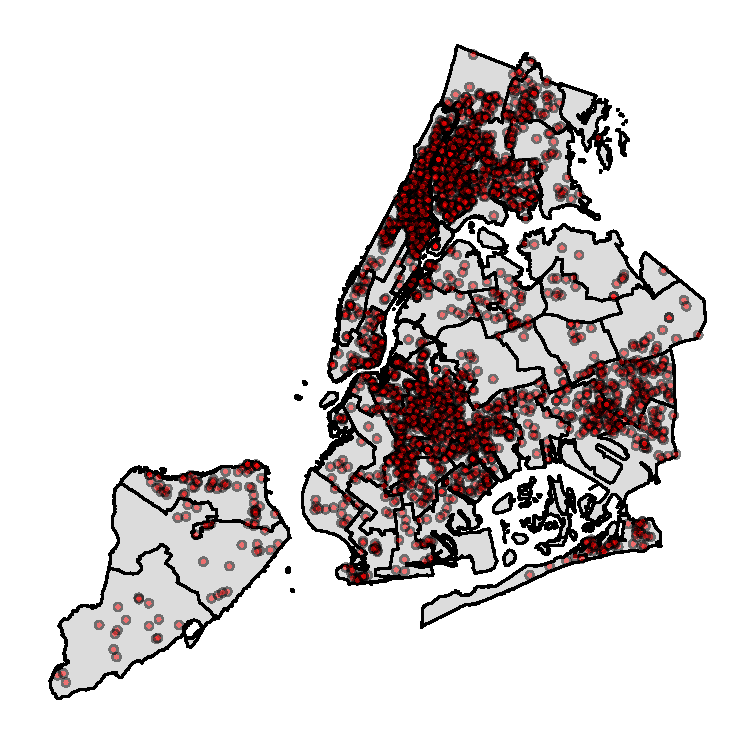
\includegraphics{felony_disenfranchisement_nys_files/figure-latex/citywide-map-1} 

}

\caption{\label{fig:citymap}Lost Voters on Election Day, 2017}\label{fig:citywide-map}
\end{figure}

The spatial concentration of lost voters is readily apparent. In some communities, such as Greenwich Village and Brooklyn Heights, hardly any voters were disqualified from participating in the 2017 elections. In other communities, such as Harlem and Central Brooklyn, large numbers of individuals with a demonstrated history of voting were not allowed to cast a ballot for mayor.

\hypertarget{testing-for-neighborhood-turnout-effects}{%
\subsection*{Testing for Neighborhood Turnout Effects}\label{testing-for-neighborhood-turnout-effects}}
\addcontentsline{toc}{subsection}{Testing for Neighborhood Turnout Effects}

Table \ref{tab:nhood-dist} shows the distribution of the number of lost voters by neighborhood. Most neighborhoods lost no voters at all; when a neighborhood was home to lost voters, they generally lost just one resident with a history of voting. More than two-thirds of block groups that lost any voters lost only one voter, while 45 percent of census tracts with a lost voter lost only one.

\begin{table}[H]

\caption{\label{tab:distribution-lost}\label{tab:nhood-dist} Distribution of Lost Voters}
\centering
\fontsize{10}{12}\selectfont
\begin{tabular}{ccc}
\toprule
Number of Lost Voters & Count of Block Groups & Count of Tracts\\
\midrule
0 & 4,272 & 1,008\\
1 & 1,023 & 416\\
2 & 301 & 212\\
3 & 107 & 138\\
4 & 30 & 51\\
5 & 19 & 46\\
6 & 9 & 23\\
7 & 3 & 15\\
8 & 5 & 13\\
9 & 0 & 7\\
10 & 0 & 2\\
11 & 0 & 2\\
12 & 0 & 2\\
14 & 0 & 2\\
\hline
Total & 5,769 & 1,937\\
\bottomrule
\end{tabular}
\end{table}

Because the majority of neighborhoods have either zero or one lost voter, I begin testing the effect of lost voters on neighborhood turnout using a matching model. Neighborhoods (defined as census tracts and block groups) are considered treated if they were home to \emph{at least one} lost voter in the 2017 election; they are untreated if no voters were disqualified from the election because of a felony conviction. I use a genetic match to match treated to untreated census tracts and block groups (Sekhon \protect\hyperlink{ref-Sekhon2011}{2011}), using a series of demographic and political indicators. Estimates of racial characteristics, median income, education, age, population, and share noncitizen\footnote{The Census Bureau does not make noncitizen estimates available at the block group level. As such, block groups are assigned their census tract's share noncitizen for matching purposes.} come from the Census Bureau. Party affiliation rates come from the geocoded voter file. Registration rate is calculated by dividing the number of registered voters (calculated using the voter file) by the citizen voting age population (CVAP, estimated by the Census Bureau). I include voteshare won by the winning city council representative in 2017 as a proxy for the competitiveness of the local race;\footnote{Where neighborhoods cross council district lines, this measure is the mean competitiveness faced by each voter in the neighborhood} where city council district races were more competitive, I expect that more voters will have turned out. Each treated block group is matched to 30 untreated block groups, and each treated census tract is matched with 10 other tracts. Matching is done with replacement. Tables \ref{tab:blockgroup-table} and \ref{tab:tract-table} present the results of these matches.

\hypertarget{match-output}{%
\subsubsection*{Match Output}\label{match-output}}
\addcontentsline{toc}{subsubsection}{Match Output}

\begin{table}[H]

\caption{\label{tab:block-table-chunk}\label{tab:blockgroup-table} Results of Block Group-Level Matching}
\centering
\resizebox{\linewidth}{!}{
\begin{tabular}{lllllrrrr}
\toprule
\multicolumn{1}{c}{ } & \multicolumn{2}{c}{Means: Unmatched Data} & \multicolumn{2}{c}{Means: Matched Data} & \multicolumn{4}{c}{Percent Improvement} \\
\cmidrule(l{3pt}r{3pt}){2-3} \cmidrule(l{3pt}r{3pt}){4-5} \cmidrule(l{3pt}r{3pt}){6-9}
 & Treated & Control & Treated & Control & Mean Diff & eQQ Med & eQQ Mean & eQQ Max\\
\midrule
\% Latino & 0.35 & 0.25 & 0.35 & 0.34 & 93.02 & 89.13 & 85.79 & 79.01\\
\% Non-Hispanic Black & 0.38 & 0.16 & 0.38 & 0.37 & 97.93 & 94.46 & 94.41 & 92.77\\
\% Non-Hispanic White & 0.17 & 0.40 & 0.17 & 0.18 & 96.37 & 96.06 & 95.56 & 92.99\\
Median Income & 51,792.52 & 72,612.36 & 51,792.52 & 52,768.97 & 95.31 & 93.47 & 88.62 & 74.49\\
\% With Some College & 0.64 & 0.70 & 0.64 & 0.64 & 90.75 & 94.14 & 90.29 & 80.70\\
Median Age & 35.99 & 38.34 & 35.99 & 36.25 & 89.18 & 90.84 & 85.93 & 78.56\\
Registration Rate & 1.00 & 0.94 & 1.00 & 0.98 & 59.77 & 79.89 & 72.28 & 60.42\\
\% Democrats & 0.75 & 0.65 & 0.75 & 0.75 & 96.22 & 96.52 & 94.92 & 91.02\\
\% Noncitizen & 0.16 & 0.16 & 0.16 & 0.16 & 16.58 & 14.80 & -0.06 & -60.28\\
\% Won by City Council Representative & 0.85 & 0.81 & 0.85 & 0.86 & 89.44 & 83.40 & 79.88 & 70.11\\
\bottomrule
\end{tabular}}
\end{table}

\begin{table}[H]

\caption{\label{tab:tract-table-chunk}\label{tab:tract-table} Results of Tract-Level Matching}
\centering
\resizebox{\linewidth}{!}{
\begin{tabular}{lllllrrrr}
\toprule
\multicolumn{1}{c}{ } & \multicolumn{2}{c}{Means: Unmatched Data} & \multicolumn{2}{c}{Means: Matched Data} & \multicolumn{4}{c}{Percent Improvement} \\
\cmidrule(l{3pt}r{3pt}){2-3} \cmidrule(l{3pt}r{3pt}){4-5} \cmidrule(l{3pt}r{3pt}){6-9}
 & Treated & Control & Treated & Control & Mean Diff & eQQ Med & eQQ Mean & eQQ Max\\
\midrule
\% Latino & 0.32 & 0.22 & 0.32 & 0.33 & 98.55 & 85.12 & 82.84 & 73.01\\
\% Non-Hispanic Black & 0.36 & 0.14 & 0.36 & 0.36 & 99.77 & 88.74 & 88.36 & 83.30\\
\% Non-Hispanic White & 0.19 & 0.42 & 0.19 & 0.19 & 97.50 & 96.32 & 91.29 & 79.95\\
Median Income & 53,409.42 & 71,754.50 & 53,409.42 & 55,422.41 & 89.03 & 90.83 & 84.86 & 62.84\\
\% With Some College & 0.65 & 0.71 & 0.65 & 0.65 & 90.19 & 93.52 & 88.89 & 73.01\\
Median Age & 35.76 & 38.04 & 35.76 & 35.80 & 98.12 & 74.51 & 80.56 & 71.91\\
Registration Rate & 0.94 & 0.90 & 0.94 & 0.93 & 76.63 & 86.16 & 84.24 & 71.28\\
\% Democrats & 0.74 & 0.62 & 0.74 & 0.73 & 94.58 & 94.93 & 92.05 & 82.37\\
\% Noncitizen & 0.16 & 0.17 & 0.16 & 0.17 & -123.57 & 22.48 & 8.85 & -38.79\\
\% Won by City Council Representative & 0.85 & 0.79 & 0.85 & 0.85 & 93.03 & 81.57 & 79.27 & 67.47\\
\bottomrule
\end{tabular}}
\end{table}

At both the tract and block group level, matching results in an untreated group of neighborhoods that looks substantially like the treatment group. These tables also demonstrate the striking extent to which neighborhoods with lost voters differ from the average neighborhood in New York City. Neighborhoods with lost voters are far less White,\footnote{Throughout the remainder of this project, I use White and non-Hispanic White interchangeably. Similarly, Black and non-Hispanic Black are used interchangeably, while Latino indicates Latinos of any race.} have much lower median incomes, and a larger share of voters are registered as Democrats.

After matching neighborhoods, I use a simple regression to test whether neighborhood treatment status was associated with turnout in the 2017 mayoral election. Census tract and block group level turnout rates are calculated using the geocoded voter file. Each voter's record indicates whether the voter participated in the 2017 general election, which are then aggregated to estimate the number of ballots cast in each neighborhood. The number of ballots cast is divided by the neighborhood's CVAP.

Much of the literature has discussed whether felony disenfranchisement is particularly demobilizing for eligible Black voters. I therefore include models which explore any potential difference in treatment effect in neighborhoods where a higher share of the population is Black. Table \ref{tab:match-reg} presents the results of these regression models. Robust standard errors are clustered at the level of the match (Abadie and Spiess \protect\hyperlink{ref-Abadie2019}{2019}).

\input{"../temp/table1.tex"}

When neighborhoods are measured at the block group level, a lost voter is negatively associated with turnout in the 2017 election. In block groups with lost voters, turnout was on average 0.9 percentage points lower than in comparable block groups without lost voters. This decrease, however, appears to be entirely concentrated within Black neighborhoods. When the treatment indicator is interacted with the share of the neighborhood that is non-Hispanic Black, the basic treatment dummy becomes nonsignificant. The coefficient on the interaction between treatment and share Black indicates that treated neighborhoods that are largely Black saw turnout that was as much as 2.7 percentage points lower than similar neighborhoods without lost voters. Considering that the overall turnout rate in block groups with a lost voter was just 14.6 percent, this effect is alarmingly high. For every 100 votes cast in an entirely Black block group with a lost voter, as many as 18.5 votes went uncast. The effects are slightly larger when neighborhoods are measured as block groups than as census tracts, though turnout is still significantly depressed in tracts with lost voters. This is not surprising --- because the spillover effects are likely to operate through social networks, smaller geographical units are likely to be more affected.

\hypertarget{testing-intensity-effects}{%
\subsubsection*{Testing Intensity Effects}\label{testing-intensity-effects}}
\addcontentsline{toc}{subsubsection}{Testing Intensity Effects}

Matching methodologies, of course, only allow us to test the effect of being treated --- here, losing any voter for the 2017 election. The models above do not allow for different effects on turnout based on \emph{how many} voters a neighborhood lost, potentially understating the impact of felony disenfranchisement in the most hard-hit communities. In Table \ref{tab:trad-reg} below, I adopt a standard ordinary least squares regression to investigate whether lost voters are associated with lower turnout rates in the 2017 election. This regression uses the same covariates used in the matching procedure described above. Robust standard errors are clustered by city council district.\footnote{Where neighborhoods cross city council district lines, they are assigned the district in which most of their voters live for clustering purposes.}

\input{"../temp/table2.tex"}

The results presented in Table \ref{tab:trad-reg} align closely with the estimated effect from the matching model. Lost voters are generally associated with lower turnout (each missing voter in a block group reduces that neighborhood's turnout by about 0.82 percentage points), but Models 2 and 4 again make clear that this effect is concentrated in Black neighborhoods. In neighborhoods where most residents are Black, each lost voter is associated with a turnout decrease of up to 1.87 percentage points. The neighborhoods most affected by felony disenfranchisement are neighborhoods where incarceration patterns overlap with Black communities.

The block groups where these depressive effects are not randomly distributed throughout the city. They are highly spatially concentrated in Central Brooklyn, Eastern Queens, and Harlem. Figure \ref{fig:postest} applies the coefficient on \(Lost\ Voters \times Share\ Black\) from Model 2 in Table \ref{tab:trad-reg} to the city's block groups. The estimated depressive effect is \(-0.019\times Lost\ Voters \times Share\ Black\).

\begin{figure}[H]

{\centering 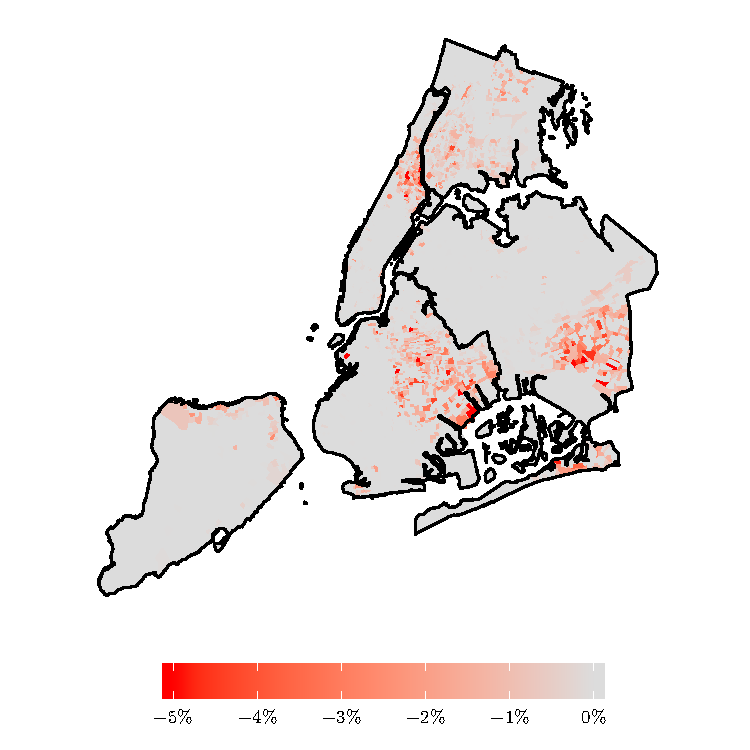
\includegraphics{felony_disenfranchisement_nys_files/figure-latex/postest-map-1} 

}

\caption{\label{fig:postest}Estimated Depressive Effect of Felony Disenfranchisement}\label{fig:postest-map}
\end{figure}

\hypertarget{toward-a-causal-estimation}{%
\subsubsection*{Toward a Causal Estimation}\label{toward-a-causal-estimation}}
\addcontentsline{toc}{subsubsection}{Toward a Causal Estimation}

As the analyses above make clear, neighborhoods with lost voters saw substantially lower turnout in the 2017 mayoral election than neighborhoods without lost voters. The possibility remains, however, that treated neighborhoods systematically differ from untreated neighborhoods in ways that cannot be accounted for using the available data. If that were the case, we would expect that these treated neighborhoods would have lower turnout regardless of whether they lost a voter. As the analysis that follows shows, this is not the case: prior to losing a voter, treated neighborhoods did not have systematically lower turnout than other neighborhoods.

I begin by restricting the set of neighborhoods to only neighborhoods that, on election day in 2016, had no lost voters. This process is the inverse of the process described above: I identify all individuals who were in prison or on parole on November 8\textsuperscript{th}, 2016, who had cast a ballot between 2006 and 2015. These individuals' home neighborhoods are removed from the subsequent analysis. I then use the genetic match algorithm discussed above to match neighborhoods with a lost voter in 2017 to neighborhoods with no lost voters in 2017. These neighborhoods, therefore, were \emph{newly} home to lost voters. If lost voters have no effect on neighborhood turnout, we would expect these treated neighborhoods to have lower turnout in both 2016 --- before they lost a voter --- and in 2017, after a voter was disenfranchised. In 2017, 1,497 neighborhoods had a lost voter; of these, 326 had no lost voters in 2016 and are included here. The original set of control block groups included 4,272 neighborhoods with no lost voters; of these, 211 \emph{did} have a lost voter in 2016, and are thus excluded from this analysis.

Of course, felony disenfranchisement could structure neighborhood turnout differently for presidential and local elections. It is conceivable that the incarceration of a family member or neighbor would sour individuals on participating in local contests, but that the same individual would not read national politics through the same lens. Nevertheless, data limitations makes the 2016 election the only reasonable comparator for 2017 turnout.

Tables \ref{tab:did-match} and \ref{tab:did-match-tract} present the results of matching on these subsets of neighborhoods. As before, the match results in a highly balanced panel between treated and untreated neighborhoods.

\begin{table}[H]

\caption{\label{tab:block-table-chunk-did}\label{tab:did-match} Results of Block Group-Level Matching}
\centering
\resizebox{\linewidth}{!}{
\fontsize{10}{12}\selectfont
\begin{tabular}{lllllrrrr}
\toprule
\multicolumn{1}{c}{ } & \multicolumn{2}{c}{Means: Unmatched Data} & \multicolumn{2}{c}{Means: Matched Data} & \multicolumn{4}{c}{Percent Improvement} \\
\cmidrule(l{3pt}r{3pt}){2-3} \cmidrule(l{3pt}r{3pt}){4-5} \cmidrule(l{3pt}r{3pt}){6-9}
 & Treated & Control & Treated & Control & Mean Diff & eQQ Med & eQQ Mean & eQQ Max\\
\midrule
\% Latino & 0.35 & 0.25 & 0.35 & 0.35 & 99.00 & 96.26 & 94.92 & 85.60\\
\% Non-Hispanic Black & 0.33 & 0.16 & 0.33 & 0.33 & 99.02 & 96.57 & 95.67 & 90.10\\
\% Non-Hispanic White & 0.21 & 0.41 & 0.21 & 0.21 & 99.61 & 94.66 & 92.61 & 82.94\\
Median Income & 55,852.62 & 73,433.49 & 55,852.62 & 56,287.76 & 97.52 & 87.85 & 86.56 & 72.89\\
\% With Some College & 0.65 & 0.71 & 0.65 & 0.65 & 99.31 & 92.25 & 87.30 & 71.15\\
Median Age & 36.17 & 38.47 & 36.17 & 36.04 & 94.37 & 62.35 & 72.27 & 69.84\\
Registration Rate & 0.98 & 0.94 & 0.98 & 0.95 & 25.09 & 46.49 & 42.16 & 33.06\\
\% Democrats & 0.73 & 0.64 & 0.73 & 0.73 & 95.94 & 94.99 & 93.62 & 86.68\\
\% Noncitizen & 0.17 & 0.16 & 0.17 & 0.17 & 63.46 & 75.01 & 66.85 & 45.71\\
\% Won by City Council Representative & 0.85 & 0.80 & 0.85 & 0.85 & 88.19 & 83.99 & 78.23 & 67.54\\
\bottomrule
\end{tabular}}
\end{table}

\begin{table}[H]

\caption{\label{tab:tract-chunk-did}\label{tab:did-match-tract} Results of Tract-Level Matching}
\centering
\resizebox{\linewidth}{!}{
\fontsize{10}{12}\selectfont
\begin{tabular}{lllllrrrr}
\toprule
\multicolumn{1}{c}{ } & \multicolumn{2}{c}{Means: Unmatched Data} & \multicolumn{2}{c}{Means: Matched Data} & \multicolumn{4}{c}{Percent Improvement} \\
\cmidrule(l{3pt}r{3pt}){2-3} \cmidrule(l{3pt}r{3pt}){4-5} \cmidrule(l{3pt}r{3pt}){6-9}
 & Treated & Control & Treated & Control & Mean Diff & eQQ Med & eQQ Mean & eQQ Max\\
\midrule
\% Latino & 0.31 & 0.22 & 0.31 & 0.30 & 94.34 & 86.10 & 84.77 & 75.82\\
\% Non-Hispanic Black & 0.25 & 0.12 & 0.25 & 0.25 & 99.28 & 89.75 & 86.62 & 77.90\\
\% Non-Hispanic White & 0.29 & 0.44 & 0.29 & 0.28 & 97.02 & 87.45 & 77.73 & 61.67\\
Median Income & 59,990.43 & 72,565.90 & 59,990.43 & 61,973.89 & 84.23 & 78.35 & 76.98 & 66.57\\
\% With Some College & 0.67 & 0.71 & 0.67 & 0.66 & 96.86 & 86.51 & 83.73 & 76.55\\
Median Age & 36.36 & 38.23 & 36.36 & 36.39 & 98.60 & 73.15 & 69.00 & 42.11\\
Registration Rate & 0.92 & 0.90 & 0.92 & 0.91 & 10.68 & 64.27 & 63.46 & 56.35\\
\% Democrats & 0.69 & 0.62 & 0.69 & 0.68 & 91.23 & 90.06 & 87.35 & 76.31\\
\% Noncitizen & 0.18 & 0.17 & 0.18 & 0.18 & 78.09 & 73.55 & 62.03 & 48.36\\
\% Won by City Council Representative & 0.83 & 0.79 & 0.83 & 0.83 & 99.91 & 75.59 & 65.98 & 38.91\\
\bottomrule
\end{tabular}}
\end{table}

In Table \ref{tab:did-reg}, I present the out come of a simple least squares regression on this subset of block groups and tracts. In both models, D(2017) indicates that across the board turnout in 2017 was far lower than in 2016. D(Treat) can be understood as the difference between treated and control neighborhoods in the 2016 election. In Model 1, the treated and control neighborhoods did not have statistically significantly different turnout in the 2016 election; Model 2 indicates that treated census tracts had slightly \emph{higher} turnout prior to intervention. D(Treat) \(\times\) D(2017) is the coefficient of most interest here: it indicates whether, after treatment, treated neighborhoods turned out at lower rates than similar neighborhoods. In Model 1, this coefficient is negative and statistically significant, and is very similar to the coefficients reported in Tables \ref{tab:match-reg} and \ref{tab:trad-reg}. Model 1 in Table \ref{tab:did-reg} indicates that, in the first election after the removal of a voter, a neighborhood's turnout rate decreased by 2.6 percentage points. The relationship does not hold for tracts (suprisingly, treated tracts turned out at higher rates both before and after treatment than control tracts).

\input{"../temp/table1111.tex"}

Table \ref{tab:did-reg} makes clear that the removal of lost voters likely has a causal effect on neighborhoods' turnout rates. It is worth noting that this is the treatment effect on the treated --- which is to say, it is estimated using only neighborhoods with no lost voters in 2016. These neighborhoods may differ from neighborhoods that had lost voters in both 2016 and 2017. Indeed, neighborhoods that consistently have lost voters are more likely to be the places most impacted by policing patterns. Among block groups that had a lost voter in 2017, those who had no lost voters in 2016 were higher-income (\$51k versus \$56k), had higher shares non-Hispanic White (16 percent versus 21 percent), a lower share non-Hispanic Black (39 percent versus 33 percent), and a smaller share were registered as Democrats (76 percent versus 73 percent).\footnote{Each of these differences are significant at the 99 percent confidence level.} Each of these differences were even more magnified when comparing tracts included in this analysis to all tracts with lost voters in 2017.

Of particular note is the lower share of the population in these neighborhoods that is Black. The analyses above indicate that neighborhoods with more Black residents respond the most strongly to felony disenfranchisement. The set of neighborhoods in this section, therefore, are likely among the least likely to see this relationship. Nevertheless, that this relationship can be detected at the block group level lends credence to the causal relationship between lost voters and depressed turnout.

\hypertarget{discussion}{%
\subsection*{Discussion}\label{discussion}}
\addcontentsline{toc}{subsection}{Discussion}

During the 2017 mayoral election, felony disenfranchisement laws were responsible for removing an estimated 2,518 voters from New York City neighborhoods. The spatial concentration of these lost voters is striking, as demonstrated in Figure \ref{fig:citywide-map}, and the systematic removal of voters from these neighborhoods is troubling. However, more than one million votes were cast in the general election of 2017. Although felony disenfranchisement rules have implications for the individuals targeted by them, the removal of such a small number of voters --- concentrated though they are --- is unlikely to have large implications on its own.

As this analysis makes clear, however, felony disenfranchisement reaches beyond the individuals who are incarcerated. Previous literature has established that felony disenfranchisement impacts Black turnout at the state level, but this analysis demonstrates that these demobilizing effects intersect with geographical space to systematically depress the vote in neighborhoods where voters are being sent to prison. As discussed above, these neighborhoods have far lower incomes than the rest of the city: the median income of block groups without any lost voters is more than 40 percent higher than the median income of block groups with lost voters. Similarly, just 17 percent of individuals in the average block group with a lost voter were White, compared with 40 percent of the population in other block groups. Felony disenfranchisement has spillover effects on neighborhood turnout, and these neighborhoods systematically differ from the rest of the city's population. The effects are concentrated in neighborhoods where the most marginalized members of society live. These highly concentrated spillover effects are cause for major concern.

Of equal concern is the apparent concentration of these effects in Black neighborhoods. Both Tables \ref{tab:match-reg} and \ref{tab:trad-reg} indicate that once the lost voter indicator is interacted with the share of a neighborhood that is non-Hispanic Black, the lost voter indicator is either nonsignificant or significant and positive. This means that lost voters have no spillover effects in neighborhoods with small Black populations. Understanding the magnitude of this finding is important. In New York City, there are 165 block groups where the Black community makes up more than 90 percent of the population, with an average of 821 voting age citizens. Model 2 of Table \ref{tab:match-reg} indicates that, in a block group that is 90 percent Black with a citizen voting age population of 821, having any lost voter reduced turnout by 20 ballots. Conversely, in a block group with the same voting age population that is just 10 percent Black, the loss of any voter decreased turnout by just 2.2 ballots.

The standard OLS regression results tell a similar story: in our average block group that is 90 percent Black, each lost voter cost the neighborhood 13.9 ballots. In block groups of the same size where the population is just 10 percent Black, lost voters cost the neighborhood just 1.5 ballots --- hardly more votes than the lost voter herself.

Why do lost voters in Black neighborhoods have such large spillover effects, when lost voters in predominantly non-Black neighborhoods do not? Much of the previous literature in this space establishes that individuals who have negative interactions with the government are less likely to choose to interact with the state in the future --- that these interactions have large ``interpretive effects'' (Pierson \protect\hyperlink{ref-Pierson1993}{1993}). Lerman and Weaver (\protect\hyperlink{ref-Lerman2013}{2013}), for instance, shows that neighborhoods where there are many police stops that involve searches or use of force use 311 services less frequently. Weaver and Lerman (\protect\hyperlink{ref-Weaver2010}{2010}) argues that interactions with the criminal justice system changes how individuals understand both their identities as citizens and the nature of governmental structures. Similarly, Weaver and Lerman (\protect\hyperlink{ref-Weaver2014}{2014}) tells us that those who have had contact with the criminal justice system consider political participation not just unfruitful but rather ``as something to be actively avoided'' (16). It is perhaps unsurprising that the negative spillover effects are largest in neighborhoods where police presence and criminal justice involvement is most keenly (and unfairly) felt; namely, in plurality and majority Black neighborhoods.

Individuals who live in neighborhoods where police activity is relatively limited may interpret the incarceration of a neighbor as a largely individual phenomenon. If it is understood as an isolated or individual event, voters in these neighborhoods who are not incarcerated are not likely to update their view of the state. They may draw no connections between their neighbor's imprisonment and their own efficacy as a voter. In the neighborhoods where policing is most prevalent --- often, lower-income Black communities --- the incarceration of a neighbor might not be interpreted so individualistically. It may, rather, be interpreted as another reminder of the government's unfairness. If a would-be voter finds herself soured on political participation because of her neighbor's incarceration, she may be less likely to cast a ballot.

This finding mirrors White (\protect\hyperlink{ref-White2019}{2019}), which finds that brief jail spells decrease future participation more for Black individuals than for White individuals. This is perhaps unsurprising. A large body of research indicates that, even after controlling for various sociodemographic characteristics and interactions with the police, Black Americans have far more negative views of the criminal justice system than White Americans (e.g.~Browning and Cao \protect\hyperlink{ref-Browning1992}{1992}; Hurwitz and Peffley \protect\hyperlink{ref-Hurwitz2005}{2005}; Henderson et al. \protect\hyperlink{ref-Henderson1997}{1997}; Wu, Sun, and Triplett \protect\hyperlink{ref-Wu2009}{2009}). Experience with the criminal justice system is less likely to be viewed in isolation (and therefore more likely to affect voting patterns) in Black neighborhoods. There is therefore strong reason to suspect that the concentrated depressive effects of felony disenfranchisement in Black neighborhoods arise from these distinct interpretations of the act of incarceration by the state.

For decades, scholars have detailed the problems associated with poor and segregated urban neighborhoods (Wilson \protect\hyperlink{ref-Wilson1990}{1990}). More recent work has begun to interrogate the ways in which the increasing reach of the carceral state shapes the economic and political behavior of individuals caught up in the criminal justice system and their community members. Much of this work, however, has focused on either the impacts of living in marginalized communities (by measuring health and economic impacts) or has not accounted for the importance of physical space (by focusing only on proximal social, and not geographic, contact with directly impacted individuals). This analysis allows us to understand the implications for living in a neighborhood where individuals likely to cast a ballot are not allowed to because of a felony conviction. I find that neighborhoods that are home to lost voters --- and particularly neighborhoods with large Black populations --- systematically turn out for local elections at lower rates than otherwise similar neighborhoods.

This has major ramifications for how we understand the political positioning of the minority neighborhoods most impacted by overpolicing and incarceration. In the case of the 2017 election, there were likely no electoral consequences: Bill de Blasio won reelection handily, and neighborhoods with lost voters overwhelmingly supported his candidacy. A lack of electoral consequences in 2017, however, should not be interpreted to mean that the disparate and concentrated depressive effects of felony disenfranchisement never have implications for who is elected to local office. As Hajnal and Trounstine (\protect\hyperlink{ref-Hajnal2005}{2005}) shows, racial turnout differentials can have real consequences for city politics.

Moreover, we cannot conclude that depressed turnout in these neighborhoods in 2017 had no impact on their representation. City council members representing these neighborhoods, for instance, may determine that pushing for policies popular with these constituents (such as stricter police oversight) will not garner enough votes to make such a fight worthwhile. Although spillover effects from felony disenfranchisement may not have changed who won power in 2017, it very possibly altered how those individuals \emph{held} and \emph{used} their power.

Felony disenfranchisement laws, originally adopted during Jim Crow, have taken on a new life in the era of mass incarceration. Abundant research has demonstrated the pernicious ways in which overincarceration dogs the lives of poor and non-White Americans. As this study shows, however, the neighborhoods bearing the brunt of felony disenfranchisement are also seeing their political power diminished through reduced turnout. The interlocking nature of racioeconomic segregation, politicing patterns, and felony disenfranchisement all combine to undermine the political power of marginalized communities in New York City.

\pagebreak

\hypertarget{executive-order-181-and-turnout-in-2018}{%
\section{Executive Order 181 and Turnout in 2018}\label{executive-order-181-and-turnout-in-2018}}

Prior to 2018, New Yorkers convicted of felony offenses and sentenced to prison were disenfranchised until they had completed all terms of their sentence --- their period of incarceration as well as any parole term. For New Yorkers on life parole or sentenced to life in prison, this law resulted in effective lifetime disenfranchisement. New Yorkers sentenced to felony probation, on the other hand, did not lose their voting rights.

On April 18\textsuperscript{th}, 2018, Governor Andrew Cuomo signed Executive Order 181 which effectively ended the disenfranchisement of New Yorkers on parole. Such a move was of course good for the communities in which parolees live; as discussed above, the disenfranchisement of voters has large spillover effects in the neighborhoods in which these lost voters are concentrated. The change in policy is also beneficial for felony probationers: despite the fact that probationers do not formally lose their voting rights, there is evidence that confusion around the law contributes to \emph{de facto} disenfranchisement among probationers (Drucker and Barreras \protect\hyperlink{ref-Drucker2005}{2005}). The executive order is a promising step: by changing the policy to allow all New York citizens living in their communities to cast a ballot, the move has the potential to both re-enfranchise the nearly 30,000 New Yorkers on parole living in the community and to clarify the rules about who is eligible to vote.

Of course, re-extending the right to vote is only the first step. As previous literature has established, interactions with the criminal justice system leaves residents less likely to vote in the future (White \protect\hyperlink{ref-White2019}{2019}). As Burch (\protect\hyperlink{ref-Burch2011}{2011}) and others have shown, moreover, turnout rates among the formerly incarcerated are extremely low. Formal disenfranchisement policy, the literature has made clear, is just one piece of an interlocking system that serves to disenfranchise minority and marginalized voters (see, for instance, Fraga \protect\hyperlink{ref-Fraga2018}{2018}). To address \emph{only} the formal laws contributing to disenfranchisement without also interrogating the efficacy of any policy change to boost participation risks leaving much of the system of effective disenfranchisement undisturbed.

There is reason to believe that the executive order may have increased the political participation of formerly disenfranchised individuals. Prior to the policy change, formerly incarcerated individuals had their voting rights restored automatically upon the completion of their parole term. New York's correction code provides no more guidance other than that ``upon a person's discharge from community supervision, the department shall notify such person of his or her right to vote and provide such person with a form of application for voter registration'' (Section 75 of the New York State Correction Law). Shortly after the implementation of the executive order, Acting Deputy Commissioner for Community Supervision Ana Enright sent a memorandum to New York State parole officers detailing the Department of Corrections' new approach.\footnote{Link: \url{https://nyassembly.gov/member_files/139/webdocs/82103.pdf}} The memorandum directs all parole officers to present parolees with voter registration forms and to explain their purpose. Parole officers were also instructed to offer any assistance needed, including help filling out the registration form. In addition to these directives, the memorandum communicates that voter registration is to receive ``high priority attention,'' and it separately calls the program ``a \textbf{priority} initiative'' {[}emphasis in the original{]}. Thus, the executive order demands not only that re-enfranchised individuals receive in-person notification of their voting rights, but also that parole officers prioritize their registration.

In the analysis below, I examine the effect of Executive Order 181 on individuals who finished parole before October 10\textsuperscript{th}, 2018. This marked the registration deadline for the 2018 general election, in which New Yorkers cast ballots in both gubernatorial and U.S. senatorial contests (as well as other down-ballot races).

I focus only on the individuals who would have been eligible to cast a ballot whether or not the executive order was signed. This is, of course, only a subset of the individuals who were impacted by Executive Order 181 --- many of the individuals who had their voting rights restored were still on parole on Election Day, and therefore were eligible to vote only because of the rules change. However, by focusing on individuals who would have been eligible to vote either way, I can test whether rights restoration prior to parole discharge serves as an effective encouragement of post-supervision participation.

\hypertarget{identifying-parolees-whose-rights-were-restored}{%
\subsection*{Identifying Parolees Whose Rights Were Restored}\label{identifying-parolees-whose-rights-were-restored}}
\addcontentsline{toc}{subsection}{Identifying Parolees Whose Rights Were Restored}

Following Executive Order 181, the Department of Corrections and Community Supervision began indicating on their online Parolee Lookup Tool whether a parolee had her voting rights restored. By using the identification number provided from the parolee public records request and this website, I was able to identify individuals who had their voting rights restored.\footnote{Not all parolees listed in the public records request data are included in the lookup tool. For individuals who finished parole between January 1\textsuperscript{st}, 2018, and April 17\textsuperscript{th}, 2018, 1.0 percent are not in the lookup tool. For those discharged from parole between April 18\textsuperscript{th}, 2018, and January 13\textsuperscript{th}, 2019 (the latest date of the parole records), 1.2 percent of individuals are not found in the lookup tool.}

\hypertarget{trends-in-turnout}{%
\subsection*{Trends in Turnout}\label{trends-in-turnout}}
\addcontentsline{toc}{subsection}{Trends in Turnout}

Before analyzing turnout in the 2018 midterms, I begin by examining turnout in the 2016 election. It is possible that individuals discharged from parole shortly before a federal election are more likely to cast a ballot than individuals discharged earlier, whether or not their voting rights were restored. However, as Figure \ref{fig:to-16} (which plots 2016 turnout rates by month of parole discharge) makes clear, individuals discharged from parole in the final months before the 2016 presidential election were not substantially more likely to cast a ballot in the election than individuals discharged earlier. The longer an individual has been off of parole, the more likely he is to cast a ballot. For instance, of the individuals last discharged from parole in 2010, 6.6 percent cast a ballot in the 2016 election, while just 4.2 percent of those last discharged from parole in 2015 did so.\footnote{Figure \ref{fig:to-16} plots individuals' turnout by the last date of discharge from parole. Therefore, individuals discharged from parole in 2010 who reoffended and were discharged from parole again in 2015 are included only in 2015.} A quadratic curve is fitted (weighted by the number of individuals discharged each month), along with a 95 percent confidence band. This curve is fit on monthly data running from January 2010 through April 2016, and extended through October 2016.

\begin{figure}[H]

{\centering 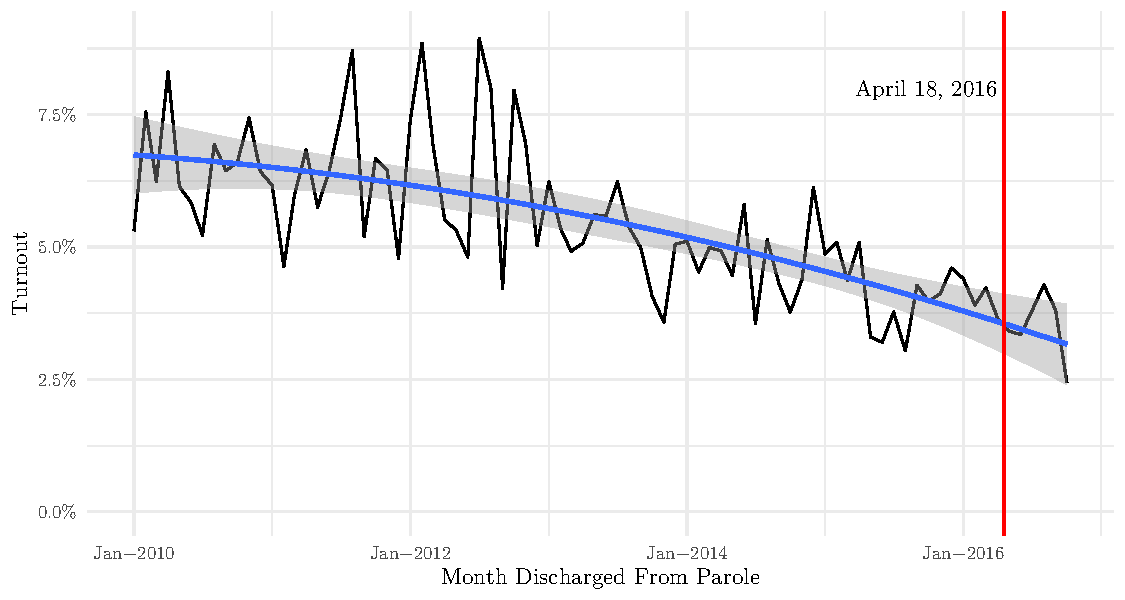
\includegraphics{felony_disenfranchisement_nys_files/figure-latex/to-16-chart-1} 

}

\caption{\label{fig:to-16}Turnout in 2016 Presidential Election}\label{fig:to-16-chart}
\end{figure}

Figure \ref{fig:to-18} plots month of parole discharge and turnout in the 2018 midterm elections. Once again, a weighted quadratic curve is fitted with a 95 percent confidence band. This curve is fit on monthly data running from January 2012 through April 2018, and extended through October 2018.

\begin{figure}[H]

{\centering 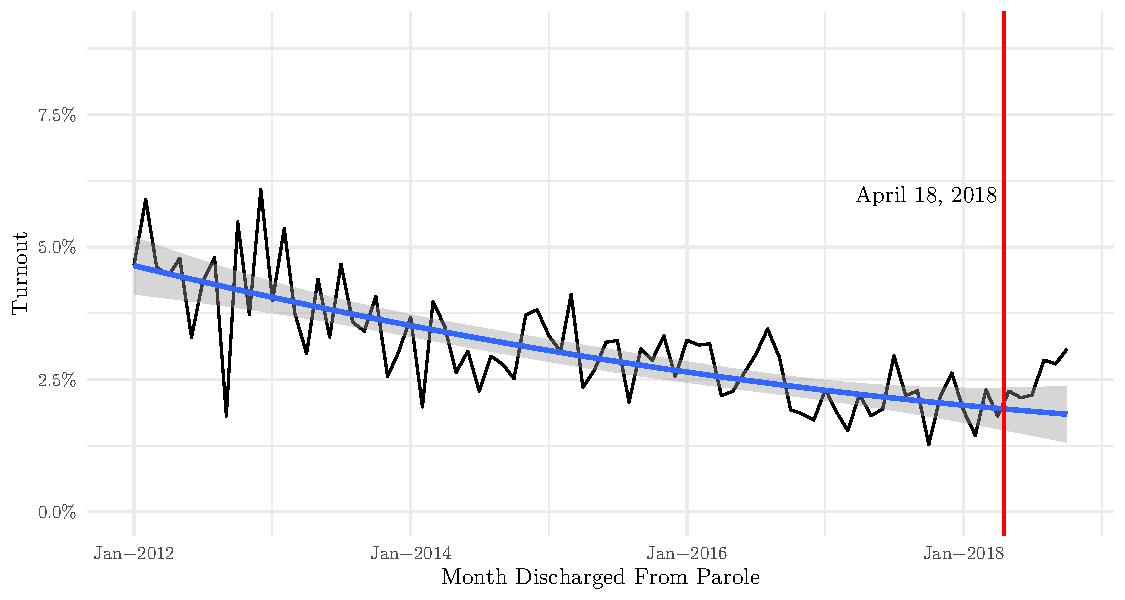
\includegraphics{felony_disenfranchisement_nys_files/figure-latex/to-18-chart-1} 

}

\caption{\label{fig:to-18}Turnout in 2018 Midterm Election}\label{fig:to-18-chart}
\end{figure}

Figure \ref{fig:to-16} does not indicate that individuals who were discharged from parole shortly before the 2016 presidential election were more likely to cast a ballot than individuals discharged earlier in the year. Figure \ref{fig:to-18}, on the other hand, indicates that New Yorkers discharged from parole in the months leading up to the 2018 election --- many of whom had their rights restored while they were still on parole --- \emph{were} more likely to participate than those discharged earlier in the year. However, Figures \ref{fig:to-16} and \ref{fig:to-18} are noisy and do not prove that the executive order increased turnout.

\hypertarget{individual-level-turnout-regressions}{%
\subsection*{Individual-Level Turnout Regressions}\label{individual-level-turnout-regressions}}
\addcontentsline{toc}{subsection}{Individual-Level Turnout Regressions}

When considered over a multi-year period, the enactment of Executive Order 181 cannot be understood as a natural experiment. The longer an individual has been off of parole, the more likely she is to cast a ballot, but only individuals recently discharged from parole were eligible to have their voting rights restored prior to discharge. For a true natural experiment to hold, an individual's probability of being ``assigned'' to treatment (here, discharged from parole after the executive order went into effect) must be uncorrelated with the outcome of interest (propensity to vote). Figures \ref{fig:to-16} and \ref{fig:to-18} indicate that this is not the case when considering individuals discharged from parole over multiple years.

However, the relationship between time-off-parole and propensity to vote is far weaker in the short term. Figure \ref{fig:to-18-recent} indicates that parole discharge date and turnout rates in the 2018 midterm election are not correlated when we limit the analysis to individuals discharged in 2017 or 2018.

\begin{figure}[H]

{\centering 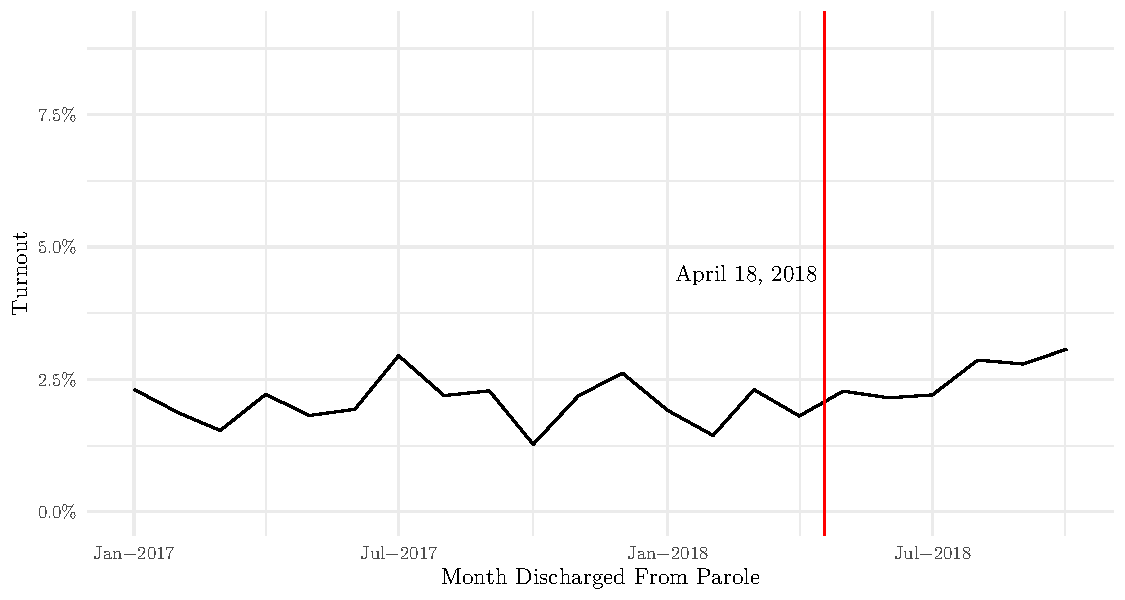
\includegraphics{felony_disenfranchisement_nys_files/figure-latex/to-18-recent-chart-1} 

}

\caption{\label{fig:to-18-recent}Turnout in 2018 Midterm Election}\label{fig:to-18-recent-chart}
\end{figure}

Formalizing this chart into an individual-level logistic model demonstrates that time since discharge is not correlated with turnout in the short run. The models in Table \ref{tab:to-18-logit-short} include individuals last discharged from parole between January 1\textsuperscript{st}, 2017, and April 17\textsuperscript{th}, 2018 --- that is to say, all individuals discharged prior to the implementation of the executive order.

\input{"../temp/table3.tex"}

The inclusion of time controls in Model 2 in Table \ref{tab:to-18-logit-short} increases the AIC. A Chi-squared test confirms that the model is not improved when controls for time are included. When we look only at individuals recently discharged from parole, the length of time an individual has been off parole is not associated with his propensity to vote.\footnote{\protect\hyperlink{appendix-a}{Appendix A} provides further corroboration that being discharged from parole in the months before an election is uncorrelated with propensity to vote by exploring turnout rates in the 2016 presidential election.}

Although Governor Cuomo signed the executive order on April 18, 2018, an examination of the individuals whose rights were ultimately restored indicates that the program did not go into full effect until later in May. Figure \ref{fig:restoration-chart} plots the share of individuals discharged from parole each day in the spring of 2018. It is not until May 18\textsuperscript{th} that parolees consistently had their voting rights restored prior to discharge.

\begin{figure}[H]

{\centering 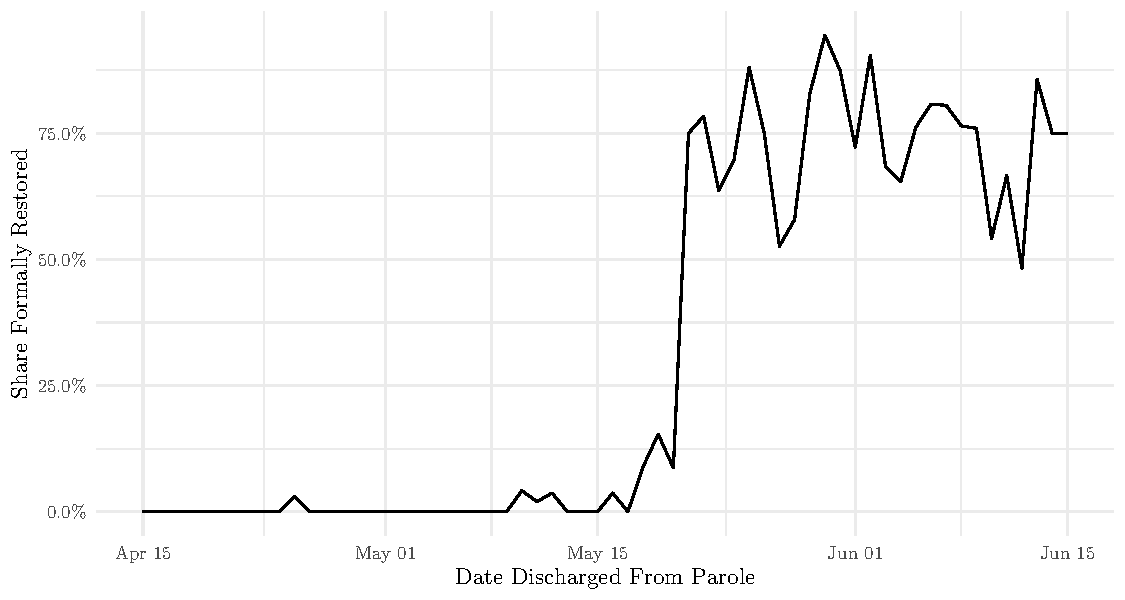
\includegraphics{felony_disenfranchisement_nys_files/figure-latex/restoration-chart-chunk-1} 

}

\caption{\label{fig:restoration-chart}Share of Discharged Parolees Whose Voting Rights Were Restored Prior to Discharge}\label{fig:restoration-chart-chunk}
\end{figure}

Although it perhaps seems counterintuitive to throw out many of our observations, ignoring all individuals last discharged from parole prior to 2017 give us an important asset: it allows us to conceptualize Executive Order 181 as a natural experiment. Whether an individual was discharged from parole before or after May 18\textsuperscript{th}, 2018, is akin to a randomly assigned treatment. Individuals who were discharged from parole prior to the implementation of the executive order are part of the ``control group'', while individuals discharged after are ``treated'' by the policy change. Because Table \ref{tab:to-18-logit-short} shows that discharge date from parole is uncorrelated in the short term with an individual's propensity to vote, any observed difference in turnout between individuals discharged before and after late May can therefore be attributed to the executive order.

To further demonstrate the usefulness of discharge date as an intend-to-treat indicator, Table \ref{tab:demo-rd} shows the demographic characteristics of individuals in the control group (those discharged between January 1st, 2017, and May 17th, 2018) and the intend-to-treat group (those discharged between May 18th and October 12th, 2018). With the exception of age, the control and intend-to-treat groups are statistically indistinguishable from one another, further demonstrating the validity of the natural experiment conceptualization. The control group is, on average, slightly older, which Table \ref{tab:to-18-logit-short} indicates makes them slightly more likely to vote. To the extent our control group perhaps has a slightly higher propensity to vote than our intend-to-treat group our setup is biased against finding a significant increase due to the executive order.

\input{"../temp/table_whatever2.tex"}

In Table \ref{tab:to-18-logit}, I present the results of an individual-level logistic regression exploring whether individuals who were discharged on or after May 18\textsuperscript{th}, 2018, turned out at higher rates than those discharged earlier. The models include all individuals discharged from parole between January 1\textsuperscript{st}, 2017, through October 10\textsuperscript{th}, 2018 (the registration deadline in New York State).

\input{"../temp/table4.tex"}

Model 1 in Table \ref{tab:to-18-logit} formalizes the trend presented in Figure \ref{fig:to-18-recent-chart} by controlling only for whether an individual was discharged after Executive Order 181 went into effect. Model 2 also controls for individual-level characteristics: sex, age on November 6\textsuperscript{th}, 2018, and race. Model 3 adds sentence-specific information to Model 2: the amount of time the individual spent on parole, and the class(es) of felony for which they were convicted. Table \ref{tab:to-18-logit} makes clear that formerly incarcerated men were far less likely to vote than formerly incarcerated women; that older formerly incarcerated individuals were more likely to cast a ballot; and individuals who spent longer on parole were more likely to participate in the midterm election.

Models 2 and 3 also indicate that individuals discharged from parole after the executive order went into effect were more likely to cast a ballot than those discharged earlier. Exponentiating the coefficients on D(Discharged After EO 181) indicates that Executive Order 181 raised the turnout rate among all formerly disenfranchised individuals by between 31.2 and 31.8 percent.

\hypertarget{instrumental-variables-approach}{%
\subsection*{Instrumental Variables Approach}\label{instrumental-variables-approach}}
\addcontentsline{toc}{subsection}{Instrumental Variables Approach}

Table \ref{tab:to-18-logit} indicates that executive order was successful at increasing turnout among all formerly disenfranchised individuals. Although this is important information for policymakers and advocates hoping to increase the political representation of formerly incarcerated individuals as a whole, it does not shed light on the extent to which rights restoration increased the propensity to vote for the individuals who actually received the treatment. To answer that question, we must specifically control for whether an individual actually had his rights restored before he was discharged from parole --- not simply whether he was discharged after the policy change.

Investigating the causal effect of rights restoration using the natural experiment conceptualization introduces a complication: not all individuals who were discharged from parole after Executive Order 181 went into effect had their rights restored --- that is to say, not all individuals assigned to the treatment group ``complied.'' Moreover, there is reason to suspect that compliance is correlated with propensity to vote.

An individual's propensity to vote can be expressed using the following equation:
\[ Y_i =  b_0 + b_{1}X_{1i} + b_{2}X_{2i} + b_{3}Z{i}+ \epsilon_{i} \]
Where \emph{Y\textsubscript{i}} is 1 if individual \emph{i} cast a ballot, \emph{X\textsubscript{1i}} is the probability that individual \emph{i} was eligible to have his rights restored prior to discharge from parole, and \emph{X\textsubscript{2i}} is 1 if individual \emph{i} actually had his rights restored prior to discharge from parole. \emph{Z} is a vector of other factors (such as age and race) known to influence voter turnout. Given that we cannot observe \emph{X\textsubscript{1i}}, we could simply choose to ignore it. Doing so, however, will result in consistent regression coefficients only if \emph{X\textsubscript{1i}} and \emph{X\textsubscript{2i}} (that is, eligibility to have rights restored, and actual restoration) are uncorrelated or if \emph{b\textsubscript{1}} is uncorrelated with an individual's propensity to vote (\emph{Y\textsubscript{i}}).

Neither of these assumptions are valid: firstly, an individual's eligibility to have her rights restored is certainly correlated with whether or not they actually were restored because the executive order required that all eligible individuals have their voting rights restored. Secondly, an individual's likelihood of having his rights restored is probably correlated with his natural propensity to vote. Individuals who were discharged from parole but are not U.S. citizens, for instance, did not having voting rights restored (or, in this case, granted) after the executive order went into effect. This ineligibility to have voting rights granted is of course correlated with these individuals' propensity to vote: non-citizens cannot cast ballots in elections in New York State. Although the available data does not indicate whether individuals were eligible to have their rights restored, we can examine the demographic differences between individuals who had their rights restored and those who did not.

\input{"../temp/table_whatever.tex"}

Table \ref{tab:demos-restorees} makes clear that the restoration of voting rights (``compliance'') is strongly correlated with certain demographics that are also linked to propensity to vote. Men, for instance, were less likely to have their rights restored than women, and Table \ref{tab:to-18-logit} above indicates that men who have been on probation are less likely to vote than women. Similarly, Latinos made up more than a third of individuals whose rights were not restored, but just 19 percent of individuals who did have voting rights restored. This is likely a reflection of citizenship status. Table \ref{tab:demos-restorees} indicates that \emph{b\textsubscript{1}} is very probably correlated with \emph{Y}. An approach in which is we regress turnout on a dummy indicating rights restoration is therefore inappropriate: such an approach cannot tell whether rights restoration \emph{caused} turnout to increase, or whether it simply identifies individuals with a higher propensity to vote.

The standard way of dealing with such a problem is an instrumental variables approach (Angrist, Imbens, and Rubin \protect\hyperlink{ref-Angrist1996}{1996}). Such an approach has been widely used in the context of voter turnout (e.g.~Ansolabehere, Iyengar, and Simon \protect\hyperlink{ref-Ansolabehere1999}{1999}; Gerber and Green \protect\hyperlink{ref-Gerber2000}{2000}; Milligan, Moretti, and Oreopoulos \protect\hyperlink{ref-Milligan2004}{2004}; Lassen \protect\hyperlink{ref-Lassen2004}{2004}; Sondheimer and Green \protect\hyperlink{ref-Sondheimer2010}{2010}). A valid instrumental variable must satisfy two criteria: it must be correlated with the right-hand-side (endogenous) variable of interest, and it must be uncorrelated with dependent variable (except via the endogenous variable).

In this case, such a variable is readily at hand. The likelihood that an individual had his voting rights restored is (in part) a function of whether he was discharged from parole after Executive Order 181 took effect. As demonstrated above, date of discharge from parole is not correlated with propensity to vote when we limit our analysis to individuals discharged from parole in 2017 or 2018. A dummy variable indicating whether an individual was discharged after the executive order was implemented, therefore, satisfies the criteria for an instrumental variable.

Two-stage least squares models allow us to leverage the random assignment of parole discharge date to identify the causal effect of rights restoration on the treated population --- what is often described as the ``local average treatment effect.'' The nature of our dependent variable (voting), instrumented variable (rights restoration), and instrument (discharge from parole before or after EO 181 went into effect) pose a challenge: each are binary values that can either be equal to 0 or 1. Linear models such as two-stage least squares do not ensure that the predicted probability of voting will fall on the {[}0, 1{]} interval. Although Angrist (\protect\hyperlink{ref-Angrist2001}{2001}) and Angrist and Pischke (\protect\hyperlink{ref-Angrist2008}{2008}) argue that in practice this limitation is usually trivial, the possibility remains that the linear model results in unacceptable misspecification. Some research (e.g.~Gerber and Green \protect\hyperlink{ref-Gerber2000}{2000}; Green and Shachar \protect\hyperlink{ref-Green2000}{2000}; Lassen \protect\hyperlink{ref-Lassen2004}{2004}) using instrumental variables in the context of a binary vote-no vote framework has employed a two-stage probit (2S probit) model to avoid the constraints of the nonparametric framework. The 2S probit model specification, however, works best when the instrumented variable is continuous --- not, as in the case of rights restoration, a dichotomous variable (Dong and Lewbel \protect\hyperlink{ref-Dong2014}{2014}). The bivariate probit approach (see Wooldridge \protect\hyperlink{ref-Wooldridge2010}{2010}) is well suited for situations where the dependent variable, the instrumented variable, and instrument are all dichotomous (Terza, Bradford, and Dismuke \protect\hyperlink{ref-Terza2007}{2007}). This is especially true when the models exclude covariates and include only the dependent variable, the endogenous instrumented variable, and the instrument (Angrist \protect\hyperlink{ref-Angrist2001}{2001}).

Table \ref{tab:iv-models} presents the results of these various approaches on the question at hand. Models 1 and 2 utilize the linear two-stage least squares approach, with and without covariates. Model 3 uses the 2S probit specification (with all covariates), while Models 4 and 5 employ the bivariate probit specification (with and without covariates). For ease of comparison, I show the marginal effects of the probit models (measured at the means of the other variables).

\input{"../temp/iv_clean.tex"}

The estimates of the bivariate probit model are modestly more conservative than the two-stage least squares model. After controlling for available demographics, the bivariate probit model indicates that rights restoration prior to discharge boosted turnout by individuals who had their rights restored by around 0.74 percentage points; the two-stage least squares model estimates that it increased turnout by around 0.85 percentage points. Though these numbers may seem small, they represent relatively large gains. Just 3.0 percent of individuals who had their rights restored cast a ballot in 2018, indicating that the Executive Order increased turnout by between 32.7 and 39.5 percent.

\hypertarget{racial-variation}{%
\subsubsection*{Racial Variation}\label{racial-variation}}
\addcontentsline{toc}{subsubsection}{Racial Variation}

Although these models demonstrate that rights restoration had a generally positive effect on participation in the 2018 election, the models hide substantial variation between races. In Table \ref{tab:iv-models-r} I present the two-stage least squares and bivariate probit models on subsets of former parolees. These models include only White former parolees (Models 1 and 4), all non-White former parolees (Models 2 and 5), and only Black former parolees (Models 3 and 6). Once again, the marginal effects in the bivariate probit models are calculated at the means of the other variables.

\input{"../temp/iv_clean_race.tex"}

Table \ref{tab:iv-models-r} indicates that rights restoration prior to discharge boosted turnout among White individuals by around 1.6 percentage points. Given that just 3.3 percent of White former parolees with restored voting rights cast a ballot, this means that rights restoration \emph{nearly doubled} these individuals' likelihood of casting a ballot. We cannot determine whether rights restoration had an effect on non-White individuals: the coefficient on these estimates are small and not statistically significant.

Why would the intervention have increased turnout among White individuals and have had no effect on Black individuals? Some of this may be explained by different propensities to vote. White (\protect\hyperlink{ref-White2019}{2019}), for instance, shows that brief periods of incarceration decreases Black individuals' propensity to vote by substantially more than White individuals. She demonstrates that, prior to incarceration, Black individuals were more likely to vote, identifying ``a narrative in which targeted policing brings many Black defendants into court, including some voters (so they can be deterred), while lower arrest rates among Whites mean that the White defendant pool rarely includes voters (so there is little demobilization, because the people jailed were unlikely to vote anyway)'' (321). The inverse may hold true here: if Black individuals released from parole have a higher natural propensity to vote (even after accounting for potentially larger depressive effects from incarceration), they may be less susceptible to a policy intervention of this sort.

There is reason to believe this may be the case. Table \ref{tab:black-to} presents a series of logistic models estimating turnout in 2018 for the control group (individuals discharged from parole before the executive order went into effect), the intend-to-treat group (those discharged after the executive order), and of the treatment group (individuals whose rights were restored), testing whether Black individuals turned out at higher rates. Because Latino voters are more likely to be non-citizens (and therefore have a lower turnout rate than Black individuals), these individuals have been excluded from Models 2, 4, and 6 in case their inclusion overstates the relative propensity of Black individuals to vote.

\input{"../temp/table5.tex"}

Of the 14,155 individuals discharged from parole between January 1\textsuperscript{st}, 2017, and May 18\textsuperscript{th}, 2018, just over 6 thousand (43 percent) were Black. These Black voters were more than 50 percent more likely to vote in the midterms than the rest of the population. Even when Latinos are excluded from this group, Black individuals were still 36 percent more likely to cast a ballot. In both specifications, this higher turnout rate is significant at the 95 percent level of confidence.

Table \ref{tab:black-to} also shows, however, that among the intend-to-treat group (those discharged from parole after the executive order went into effect), Black individuals were no more likely to participate in the 2018 general election. The same is true for the treatment group --- Black individuals who had their rights restored were no more likely than other individuals to vote in 2018. The intervention, therefore, appears to have a leveling effect. Rights restoration prior to discharge seems to have no effect on future propensity to vote for Black individuals, but that does not mean they are less likely to vote than other former parolees.

\hypertarget{variable-treatment-intensity}{%
\subsubsection*{Variable Treatment Intensity}\label{variable-treatment-intensity}}
\addcontentsline{toc}{subsubsection}{Variable Treatment Intensity}

There is some reason to believe that assuming a constant treatment effect understates the true impact of Executive Order 181. Figures \ref{fig:to-18-chart} and \ref{fig:to-18-recent-chart} suggest that, among individuals who finished parole after the Executive Order went into effect, individuals who were discharged later had a higher propensity to vote. This may be due to a number of factors: for instance, parole officers may have had longer to understand and communicate the new rules. Similarly, individuals discharged later may have had more meetings with their parole officers after the policy change, giving the parole officers multiple times to encourage the individuals under study to cast a ballot. Table \ref{tab:iv-models-time} investigates turnout as a function of the number of months an individual spent on parole after having her rights restored. If the individual did not have voting rights restored, this variable takes the value 0. This variable is instrumented by the number of months an individual spent on parole after the executive order went into effect. It is coded as 0 for individuals discharged prior to the implementation of the executive order.\footnote{Because the bivariate probit specification is not appropriate when the endogenous variable is not binary, that specification is not included in Table \ref{tab:iv-models-time}.}

\input{"../temp/iv_clean_months.tex"}

Table \ref{tab:iv-models-time} indicates that variable treatment intensity matters --- individuals who spent longer on parole after they had their rights restored were more likely to vote than those whose rights were restored shortly before discharge. Table \ref{tab:iv-models-time} shows that for each month individuals spent on parole after having their rights restored, turnout increased by between 0.25 percentage points (in the 2SLS model) and 0.48 percentage points (in the 2S probit model). It is worth noting that the \emph{R\textsuperscript{2}} in Model 1 is higher than the \emph{R\textsuperscript{2}} in Model 2 in Table \ref{tab:iv-models}, indicating that allowing for a time-variant treatment effect is warranted.

Of course, with just a handful of months between the implementation of the executive order and the registration deadline for the 2018 midterms, it is impossible to know the full impact more months on parole after having one's rights restored has. One thing, however, is clear: focusing only on the individuals discharged from parole shortly after Executive Order 181 went into effect very likely underestimates the true impact it will have on parolee's propensity to vote when parolees spend more time under supervision with their rights formally restored.

\hypertarget{discussion-1}{%
\subsection*{Discussion}\label{discussion-1}}
\addcontentsline{toc}{subsection}{Discussion}

Restoring voting rights to individuals on parole is an important step toward undermining the disenfranchisement (both \emph{de jure} and \emph{de facto}) of communities of color disproportionately caught up in the criminal justice system. Prior to New York's Executive Order 181, parolees were required to wait until they finished their parole term to register to vote. That changed in 2018. On October 12\textsuperscript{th} --- the registration deadline for the 2018 midterms --- there were 21,863 active parolees whose voting rights had been restored. Without the executive order, every single one of these individuals would have been barred from participating. Though turnout among this group was low (just 792, or 3.62 percent, of these individuals successfully cast a ballot), their re-enfranchisement marks an important milestone for New York State.

As this analysis demonstrates, however, the impact of Executive Order 181 was not limited only to the individuals who would have been disenfranchised in its absence. In the case of New York State, rights restoration prior to discharge from parole is broadly successful at boosting post-supervision participation rates. In this project I estimate that rights restoration increased individuals' propensity to vote by at least 32.7 percent. This estimate, however, should be taken as a lower bound: the data indicate that individuals who spent longer on parole after having their rights restored were more likely to vote than individuals who were discharged immediately following the implementation of the Executive Order. Notably, this upward trend showed no signs of leveling off prior to the 2018 election; individuals whose rights were restored that were discharged in the fifth month after implementation voted at higher rates than those discharged after three months; those discharged after three months turned out at higher rates than those discharged in the first month.

The mechanism through which the rules change increased turnout among these individuals is not clear. Weaver and Lerman (\protect\hyperlink{ref-Weaver2010}{2010}) argues that contact with the criminal justice system restructures how individuals understand their relationship with the government and sours their desire to participate. Automatic voting rights restoration upon the completion of a sentence likely does little to combat these negative perceptions of the government. On the other hand, a parolee whose parole officer actively encourages them to register and participate may believe that the state is interested in their political participation. Such interactions may undo some of the negative socialization identified by Weaver and Lerman (\protect\hyperlink{ref-Weaver2010}{2010}).

It could also be a story of better information. As Meredith and Morse (\protect\hyperlink{ref-Meredith2015}{2015}) and Gerber et al. (\protect\hyperlink{ref-Gerber2014}{2014}) show, reminding formerly disenfranchised individuals of their restored voting rights can increase their participation (but see Meredith and Morse (\protect\hyperlink{ref-Meredith2013}{2013})). Research such as Manza and Uggen (\protect\hyperlink{ref-locked_out}{2006}) further demonstrates that many formerly incarcerated individuals wrongly believe that they are ineligible to participate. When a parolee has her voting rights restored prior to discharge --- and when her parole officer is required to inform her of that fact --- she is far more likely to be confident in her voting eligibility. The executive order likely meant that more formerly disenfranchised individuals were sure that they could cast a ballot in the 2018 election. In reality, the executive order's success at boosting turnout likely operated through multiple mechanisms.

Puzzlingly, the causal effect of pre-discharge rights restoration seems to vary based on parolees' race. Limiting the analysis to just White parolees reveals that rights restoration increased turnout by more than 90 percent. The fact that rights restoration prior to discharge appears to have no such impact on non-White or Black parolees is surprising given the magnitude of the effect for Whites. This discrepancy could be caused by a number of different factors. Firstly, Black and White individuals on parole might differ in meaningful ways that impact the successfulness of the intervention. As discussed above, Black participation among individuals discharged from parole prior to the executive order voted at significantly higher rates in 2018. The intervention was likely successful for parolees who would not have voted otherwise, but needed only a small encouragement. It may be that fewer Black former parolees are susceptible to small encouragements: they may separate more cleanly into voters and nonvoters, with fewer individuals susceptible to parole officer encouragement.

We cannot, however, rule out the possibility that racial bias among parole officers plays some role in the effectiveness of the intervention. Although parole officers may not be overtly or consciously biased toward their parolees, such bias is possible. Although there is limited literature examining racial variation in parolees' perceptions of their parole officers, there is some evidence that Black prisoners report worse inmate-staff relationships than White prisoners (Hemmens and Marquart \protect\hyperlink{ref-Hemmens2000}{2000}). Moreover, recent research indicates that street-level bureaucrats may exhibit some racial bias in the services they provide. White, Nathan, and Faller (\protect\hyperlink{ref-WHITE2014}{2014}), for instance, shows that local election administrators are less likely to respond to email questions from Latino aliases than non-Latino White aliases. There is also evidence that politicians are less likely to respond to requests from constituents of different races (Butler and Broockman \protect\hyperlink{ref-Butler2011}{2011}), and that public housing officials respond less to inquiries from Latinos (Einstein and Glick \protect\hyperlink{ref-Einstein2016}{2016}).

Parole officers may more enthusiastically encourage White parolees to register to vote and cast a ballot. This variation in encouragement would not necessarily be indicative of racial animus: it could arise from a parole officer's expectations about a parolee's political preferences. Officers are likely to provide greater encouragement to parolees they perceive to have similar political preferences. In the case of former parolees in New York State, race does serve as an effective proxy for partisanship: 82.5 percent of Black individuals discharged from parole since 2012 who participated in the 2018 election were registered Democrats; just 31.2 percent of such White individuals were registered Democrats. Ultimately, the data at hand cannot answer why the intervention succeeded at raising turnout only among White former parolees; future research must investigate why this is the case.

Re-enfranchising voters while they are still under formal supervision is obviously beneficial to the individuals who are on parole on election day; such policies allow them to make their voices heard. The case of Executive Order 181 also indicates that restoring voting rights prior to parole discharge has further benefits. In 2018, it increased turnout among individuals who were formally discharged from parole prior to the registration deadline, and therefore would have been eligible to vote even if their rights were not restored until the completion of their sentence. This is encouraging, demonstrating that the state has a unique opportunity to shape the future participation of individuals who are currently under their supervision. By restoring voting rights before individuals have completed their sentence, and by requiring parole officers to inform their parolees of their voting rights, the state can increase the political participation of a group of often-marginalized individuals, thereby increasing the democratic representation of our elections.

\hypertarget{conclusion}{%
\section{Conclusion}\label{conclusion}}

Felony disenfranchisement was originally implemented to limit the franchise of Black Americans. It continues to serve that purpose today, as Black residents of New York and states around the country are disproportionately convicted of felony offenses and imprisoned. Although we know that many of these individuals were unlikely to cast a ballot even if they had not gone to prison, the targeted disenfranchisement of a single segment of the population is deeply troubling.

As this project has demonstrated, however, the racialized penalties of felony disenfranchisement do not disappear after we control for low propensity to vote among individuals in New York City and State who are going to prison. The first half of this project attempted to refine how we think about the spatial aspects of felony disenfranchisement, and also how we identify the individuals most likely to be directly impacted by these policies. By both redefining ``lost voters'' as individuals who have a demonstrated propensity to participate and examining turnout in the physical neighborhoods they left behind, I offer a more presise accounting of the impact of these policies. What I find is troubling: neighborhoods that were home to disenfranchised individuals turn out at systematically lower rates, and this effect is concentrated in Black neighborhoods. Moreover, there is reason to believe that this is not driven by unobservable differences between neighborhoods; I also show that turnout decreased more between 2016 and 2017 in neighborhoods that newly lost voters than in neighborhoods unaffected by disenfranchisement policies.

I also offer an early investigation of the effect of Executive Order 181, which granted voting rights to most citizens on parole in New York State. This research indicates that individuals who have their rights restored prior to being discharged from parole are more likely to participate in elections, even after they are discharged. This is a welcome finding, as increasing the political participation of marginalized individuals brings us toward a fuller democracy. As with neighborhood spillover effects, however, this effect depends in great deal on the race of the parolee: rights restoration, at least in the first five months of the program in New York State, did not increase future participation among non-Whites. More research needs to be done to investigate whether this is true over a longer time period in New York, and whether it is true in other states as well.

America is becoming ever-more-diverse, and will likely be less than 50 percent non-Hispanic White by the middle of the century. As Fraga (\protect\hyperlink{ref-Fraga2018}{2018}) has documented, however, this does not necessarily mean that minorities will enjoy political power in line with their share of the population. How districts are drawn, population patterns, and rules about who can fundraise how will continue to shape the politicians we elect and the policies they enact. Breaking down \emph{de jure} (like formal disenfranchisement) and \emph{de facto} (like neighborhood spillover effects) barriers to the ballot box is of great importance. The experience in New York State over the past few years offers a better understanding of just how big this problem is, but it also offers evidence of a way forward.

\newpage

\hypertarget{appendix-a}{%
\section*{Appendix A}\label{appendix-a}}
\addcontentsline{toc}{section}{Appendix A}

In the \protect\hyperlink{instrumental-variables-approach}{Instrumental Variables Approach} section of this paper, I argue that being discharged from parole in the final months leading up to an election is uncorrelated with propensity to vote. Table \ref{tab:to-16-logit} demonstrates that individuals discharged between May 18\textsuperscript{th} -- October 14\textsuperscript{th}, 2016, did not participate at different rates in the 2016 presidential election than other formerly incarcerated individuals. Table \ref{tab:to-16-logit} includes all individuals last discharged from parole between January 1\textsuperscript{st}, 2015, and October 14\textsuperscript{th}, 2016.

\input{"../temp/table55.tex"}

Although turnout was generally higher in 2016 than in 2018 (reflecting statewide higher turnout thanks to the presidential contest), there is no evidence that being discharged in the summer of 2016 was associated with an individual's propensity to cast a ballot. The nonsignificant results from 2016 provide strong corroboration that discharge date serves as an effective instrument for rights restoration.

\newpage

\hypertarget{references}{%
\section*{References}\label{references}}
\addcontentsline{toc}{section}{References}

\setlength{\parindent}{-0.5in}
\setlength{\leftskip}{0.5in}

\noindent

\hypertarget{refs}{}
\leavevmode\hypertarget{ref-Abadie2019}{}%
Abadie, Alberto, and Jann Spiess. 2019. ``Robust Post-Matching Inference.'' \url{https://scholar.harvard.edu/spiess/publications/robust-post-matching-inference.}

\leavevmode\hypertarget{ref-Alexander2012}{}%
Alexander, Michelle. 2012. \emph{The New Jim Crow}. New York: The New Press.

\leavevmode\hypertarget{ref-Angrist2001}{}%
Angrist, Joshua D. 2001. ``Estimation of Limited Dependent Variable Models with Dummy Endogenous Regressors.'' \emph{Journal of Business \& Economic Statistics} 19 (1): 2--28. \url{https://doi.org/10.1198/07350010152472571}.

\leavevmode\hypertarget{ref-Angrist1996}{}%
Angrist, Joshua D., Guido W. Imbens, and Donald B. Rubin. 1996. ``Identification of Causal Effects Using Instrumental Variables.'' \emph{Journal of the American Statistical Association} 91 (434): 444--55. \url{https://doi.org/10.1080/01621459.1996.10476902}.

\leavevmode\hypertarget{ref-Angrist2008}{}%
Angrist, Joshua D., and Jörn-Steffen Pischke. 2008. \emph{Mostly Harmless Econometrics}. Princeton University Press. \url{https://doi.org/10.2307/j.ctvcm4j72}.

\leavevmode\hypertarget{ref-Ansolabehere1999}{}%
Ansolabehere, Stephen D., Shanto Iyengar, and Adam Simon. 1999. ``Replicating Experiments Using Aggregate and Survey Data: The Case of Negative Advertising and Turnout.'' \emph{American Political Science Review} 93 (4): 901--9. \url{https://doi.org/10.2307/2586120}.

\leavevmode\hypertarget{ref-Anzia2019}{}%
Anzia, Sarah F. 2019. ``When Does a Group of Citizens Influence Policy? Evidence from Senior Citizen Participation in City Politics.'' \emph{The Journal of Politics} 81 (1): 1--14. \url{https://doi.org/10.1086/699916}.

\leavevmode\hypertarget{ref-Behrens2003}{}%
Behrens, Angela, Christopher Uggen, and Jeff Manza. 2003. ``Ballot Manipulation and the ``Menace of Negro Domination'': Racial Threat and Felon Disenfranchisement in the United States, 18502002.'' \emph{American Journal of Sociology} 109 (3): 559--605. \url{https://doi.org/10.1086/378647}.

\leavevmode\hypertarget{ref-Bowers2009}{}%
Bowers, Melanie, and Robert R. Preuhs. 2009. ``Collateral Consequences of a Collateral Penalty: The Negative Effect of Felon Disenfranchisement Laws on the Political Participation of Nonfelons.'' \emph{Social Science Quarterly} 90 (3): 722--43. \url{https://doi.org/10.1111/j.1540-6237.2009.00640.x}.

\leavevmode\hypertarget{ref-bcj_laws}{}%
Brennan Center for Justice. 2018. ``Criminal Disenfranchisement Laws Across the United States.'' \url{https://www.brennancenter.org/criminal-disenfranchisement-laws-across-united-states}.

\leavevmode\hypertarget{ref-Browning1992}{}%
Browning, Sandra Lee, and Liqun Cao. 1992. ``The Impact of Race on Criminal Justice Ideology.'' \emph{Justice Quarterly} 9 (4): 685--701. \url{https://doi.org/10.1080/07418829200091611}.

\leavevmode\hypertarget{ref-Burch2010}{}%
Burch, Traci. 2010. ``Did Disfranchisement Laws Help Elect President Bush? New Evidence on the Turnout Rates and Candidate Preferences of Florida's Ex-Felons.'' \emph{Political Behavior} 34 (1): 1--26. \url{https://doi.org/10.1007/s11109-010-9150-9}.

\leavevmode\hypertarget{ref-Burch2011}{}%
---------. 2011. ``Turnout and Party Registration Among Criminal Offenders in the 2008 General Election.'' \emph{Law and Society Review} 45 (3): 699--730. \url{https://doi.org/10.1111/j.1540-5893.2011.00448.x}.

\leavevmode\hypertarget{ref-Burch2013}{}%
---------. 2013. ``Effects of Imprisonment and Community Supervision on Neighborhood Political Participation in North Carolina.'' Edited by Christopher Wildeman, Jacob S. Hacker, and Vesla M. Weaver. \emph{The ANNALS of the American Academy of Political and Social Science} 651 (1): 184--201. \url{https://doi.org/10.1177/0002716213503093}.

\leavevmode\hypertarget{ref-Butler2011}{}%
Butler, Daniel M., and David E. Broockman. 2011. ``Do Politicians Racially Discriminate Against Constituents? A Field Experiment on State Legislators.'' \emph{American Journal of Political Science} 55 (3): 463--77. \url{https://doi.org/10.1111/j.1540-5907.2011.00515.x}.

\leavevmode\hypertarget{ref-Cho2006}{}%
Cho, Wendy K. Tam, James G. Gimpel, and Joshua J. Dyck. 2006. ``Residential Concentration, Political Socialization, and Voter Turnout.'' \emph{The Journal of Politics} 68 (1): 156--67. \url{https://doi.org/10.1111/j.1468-2508.2006.00377.x}.

\leavevmode\hypertarget{ref-Clear2008}{}%
Clear, Todd R. 2008. ``The Effects of High Imprisonment Rates on Communities.'' \emph{Crime and Justice} 37 (1): 97--132. \url{https://doi.org/10.1086/522360}.

\leavevmode\hypertarget{ref-Dawkins2006}{}%
Dawkins, Casey J. 2006. ``Are Social Networks the Ties That Bind Families to Neighborhoods?'' \emph{Housing Studies} 21 (6): 867--81. \url{https://doi.org/10.1080/02673030600917776}.

\leavevmode\hypertarget{ref-Dong2014}{}%
Dong, Yingying, and Arthur Lewbel. 2014. ``A Simple Estimator for Binary Choice Models with Endogenous Regressors.'' \emph{Econometric Reviews} 34 (1-2): 82--105. \url{https://doi.org/10.1080/07474938.2014.944470}.

\leavevmode\hypertarget{ref-Drucker2005}{}%
Drucker, Ernest, and Ricardo Barreras. 2005. ``Studies of Voting Behavior and Felony Disenfranchisement Among Individuals in the Criminal Justice System in New York, Connecticut, and Ohio.'' Research report. Sentencing Project. \url{https://www.prisonpolicy.org/scans/sp/fd_studiesvotingbehavior.pdf}.

\leavevmode\hypertarget{ref-Einstein2016}{}%
Einstein, Katherine Levine, and David M. Glick. 2016. ``Does Race Affect Access to Government Services? An Experiment Exploring Street-Level Bureaucrats and Access to Public Housing.'' \emph{American Journal of Political Science} 61 (1): 100--116. \url{https://doi.org/10.1111/ajps.12252}.

\leavevmode\hypertarget{ref-Foladare1968}{}%
Foladare, Irving S. 1968. ``The Effect of Neighborhood on Voting Behavior.'' \emph{Political Science Quarterly} 83 (4): 516. \url{https://doi.org/10.2307/2146812}.

\leavevmode\hypertarget{ref-Fraga2018}{}%
Fraga, Bernard L. 2018. \emph{The Turnout Gap}. Cambridge, United Kingdom: Cambridge University Press. \url{https://doi.org/10.1017/9781108566483}.

\leavevmode\hypertarget{ref-Geller2014}{}%
Geller, Amanda, Jeffrey Fagan, Tom Tyler, and Bruce G. Link. 2014. ``Aggressive Policing and the Mental Health of Young Urban Men.'' \emph{American Journal of Public Health} 104 (12): 2321--7. \url{https://doi.org/10.2105/ajph.2014.302046}.

\leavevmode\hypertarget{ref-Gelman2007}{}%
Gelman, Andrew, Jeffrey Fagan, and Alex Kiss. 2007. ``An Analysis of the New York City Police Departments ``Stop-and-Frisk'' Policy in the Context of Claims of Racial Bias.'' \emph{Journal of the American Statistical Association} 102 (479): 813--23. \url{https://doi.org/10.1198/016214506000001040}.

\leavevmode\hypertarget{ref-Gerber2000}{}%
Gerber, Alan S., and Donald P. Green. 2000. ``The Effects of Canvassing, Telephone Calls, and Direct Mail on Voter Turnout: A Field Experiment.'' \emph{American Political Science Review} 94 (3): 653--63. \url{https://doi.org/10.2307/2585837}.

\leavevmode\hypertarget{ref-Gerber2003}{}%
Gerber, Alan S., Donald P. Green, and Ron Shachar. 2003. ``Voting May Be Habit-Forming: Evidence from a Randomized Field Experiment.'' \emph{American Journal of Political Science} 47 (3): 540--50. \url{https://doi.org/10.1111/1540-5907.00038}.

\leavevmode\hypertarget{ref-Gerber2014}{}%
Gerber, Alan S., Gregory A. Huber, Marc Meredith, Daniel R. Biggers, and David J. Hendry. 2014. ``Can Incarcerated Felons Be (Re)integrated into the Political System? Results from a Field Experiment.'' \emph{American Journal of Political Science} 59 (4): 912--26. \url{https://doi.org/10.1111/ajps.12166}.

\leavevmode\hypertarget{ref-Gerber2017}{}%
---------. 2017. ``Does Incarceration Reduce Voting? Evidence About the Political Consequences of Spending Time in Prison.'' \emph{The Journal of Politics} 79 (4): 1130--46. \url{https://doi.org/10.1086/692670}.

\leavevmode\hypertarget{ref-Gimpel2004}{}%
Gimpel, James G., Joshua J. Dyck, and Daron R. Shaw. 2004. ``Registrants, Voters, and Turnout Variability Across Neighborhoods.'' \emph{Political Behavior} 26 (4): 343--75. \url{https://doi.org/10.1007/s11109-004-0900-4}.

\leavevmode\hypertarget{ref-Green2000}{}%
Green, Donald P., and Ron Shachar. 2000. ``Habit Formation and Political Behaviour: Evidence of Consuetude in Voter Turnout.'' \emph{British Journal of Political Science} 30 (4): 561--73. \url{https://doi.org/10.1017/s0007123400000247}.

\leavevmode\hypertarget{ref-Griffin2005}{}%
Griffin, John D., and Brian Newman. 2005. ``Are Voters Better Represented?'' \emph{The Journal of Politics} 67 (4): 1206--27. \url{https://doi.org/10.1111/j.1468-2508.2005.00357.x}.

\leavevmode\hypertarget{ref-Guest1999}{}%
Guest, Avery M., and Susan K. Wierzbicki. 1999. ``Social Ties at the Neighborhood Level.'' \emph{Urban Affairs Review} 35 (1): 92--111. \url{https://doi.org/10.1177/10780879922184301}.

\leavevmode\hypertarget{ref-Hajnal2009}{}%
Hajnal, Zoltan. 2009. \emph{America's Uneven Democracy}. Cambridge University Press. \url{https://doi.org/10.1017/cbo9780511800535}.

\leavevmode\hypertarget{ref-Hajnal2005}{}%
Hajnal, Zoltan, and Jessica Trounstine. 2005. ``Where Turnout Matters: The Consequences of Uneven Turnout in City Politics.'' \emph{The Journal of Politics} 67 (2): 515--35. \url{https://doi.org/10.1111/j.1468-2508.2005.00327.x}.

\leavevmode\hypertarget{ref-Haselswerdt2009}{}%
Haselswerdt, Michael V. 2009. ``Con Job: An Estimate of Ex-Felon Voter Turnout Using Document-Based Data.'' \emph{Social Science Quarterly} 90 (2): 262--73. \url{https://doi.org/10.1111/j.1540-6237.2009.00616.x}.

\leavevmode\hypertarget{ref-Hemmens2000}{}%
Hemmens, Craig, and James W. Marquart. 2000. ``Friend or Foe? Race, Age, and Inmate Perceptions of Inmate-Staff Relations.'' \emph{Journal of Criminal Justice} 28 (4): 297--312. \url{https://doi.org/10.1016/s0047-2352(00)00044-1}.

\leavevmode\hypertarget{ref-Henderson1997}{}%
Henderson, Martha L., Francis T. Cullen, Liqun Cao, Sandra Lee Browning, and Renee Kopache. 1997. ``The Impact of Race on Perceptions of Criminal Injustice.'' \emph{Journal of Criminal Justice} 25 (6): 447--62. \url{https://doi.org/10.1016/s0047-2352(97)00032-9}.

\leavevmode\hypertarget{ref-Hjalmarsson2010}{}%
Hjalmarsson, Randi, and Mark Lopez. 2010. ``The Voting Behavior of Young Disenfranchised Felons: Would They Vote If They Could?'' \emph{American Law and Economics Review} 12 (2): 356--93. \url{https://doi.org/10.1093/aler/ahq004}.

\leavevmode\hypertarget{ref-Huckfeldt1979}{}%
Huckfeldt, R. Robert. 1979. ``Political Participation and the Neighborhood Social Context.'' \emph{American Journal of Political Science} 23 (3): 579. \url{https://doi.org/10.2307/2111030}.

\leavevmode\hypertarget{ref-Hurwitz2005}{}%
Hurwitz, Jon, and Mark Peffley. 2005. ``Explaining the Great Racial Divide: Perceptions of Fairness in the U.s. Criminal Justice System.'' \emph{The Journal of Politics} 67 (3): 762--83. \url{https://doi.org/10.1111/j.1468-2508.2005.00338.x}.

\leavevmode\hypertarget{ref-Kenny1992}{}%
Kenny, Christopher B. 1992. ``Political Participation and Effects from the Social Environment.'' \emph{American Journal of Political Science} 36 (1): 259. \url{https://doi.org/10.2307/2111432}.

\leavevmode\hypertarget{ref-Keyssar2009}{}%
Keyssar, Alexander. 2009. \emph{The Right to Vote: The Contested History of Democracy in the United States}. New York: Basic Books.

\leavevmode\hypertarget{ref-King2016}{}%
King, Bridgett A., and Laura Erickson. 2016. ``Disenfranchising the Enfranchised.'' \emph{Journal of Black Studies} 47 (8): 799--821. \url{https://doi.org/10.1177/0021934716659195}.

\leavevmode\hypertarget{ref-Kinsella2015}{}%
Kinsella, Chad, Colleen McTague, and Kevin N. Raleigh. 2015. ``Unmasking Geographic Polarization and Clustering: A Micro-Scalar Analysis of Partisan Voting Behavior.'' \emph{Applied Geography} 62 (August): 404--19. \url{https://doi.org/10.1016/j.apgeog.2015.04.022}.

\leavevmode\hypertarget{ref-Lassen2004}{}%
Lassen, David Dreyer. 2004. ``The Effect of Information on Voter Turnout: Evidence from a Natural Experiment.'' \emph{SSRN Electronic Journal}. \url{https://doi.org/10.2139/ssrn.475821}.

\leavevmode\hypertarget{ref-Lerman2013}{}%
Lerman, Amy E., and Vesla Weaver. 2013. ``Staying Out of Sight? Concentrated Policing and Local Political Action.'' Edited by Christopher Wildeman, Jacob S. Hacker, and Vesla M. Weaver. \emph{The ANNALS of the American Academy of Political and Social Science} 651 (1): 202--19. \url{https://doi.org/10.1177/0002716213503085}.

\leavevmode\hypertarget{ref-locked_out}{}%
Manza, Jeff, and Christopher Uggen. 2006. \emph{Locked Out: Felon Disenfranchisement and American Democracy}. New York: Oxford University Press.

\leavevmode\hypertarget{ref-Martin2003}{}%
Martin, Paul S. 2003. ``Votings Rewards: Voter Turnout, Attentive Publics, and Congressional Allocation of Federal Money.'' \emph{American Journal of Political Science} 47 (1): 110--27. \url{https://doi.org/10.1111/1540-5907.00008}.

\leavevmode\hypertarget{ref-Martin2013}{}%
Martin, Paul S., and Michele P. Claibourn. 2013. ``Citizen Participation and Congressional Responsiveness: New Evidence That Participation Matters.'' \emph{Legislative Studies Quarterly} 38 (1): 59--81. \url{https://doi.org/10.1111/lsq.12003}.

\leavevmode\hypertarget{ref-Meredith2013}{}%
Meredith, Marc, and Michael Morse. 2013. ``Do Voting Rights Notification Laws Increase Ex-Felon Turnout?'' Edited by Christopher Wildeman, Jacob S. Hacker, and Vesla M. Weaver. \emph{The ANNALS of the American Academy of Political and Social Science} 651 (1): 220--49. \url{https://doi.org/10.1177/0002716213502931}.

\leavevmode\hypertarget{ref-Meredith2015}{}%
---------. 2015. ``The Politics of the Restoration of Ex-Felon Voting Rights: The Case of Iowa.'' \emph{Quarterly Journal of Political Science} 10 (1): 41--100. \url{https://doi.org/10.1561/100.00013026}.

\leavevmode\hypertarget{ref-Miles2004}{}%
Miles, Thomas J. 2004. ``Felon Disenfranchisement and Voter Turnout.'' \emph{The Journal of Legal Studies} 33 (1): 85--129. \url{https://doi.org/10.1086/381290}.

\leavevmode\hypertarget{ref-Milligan2004}{}%
Milligan, Kevin, Enrico Moretti, and Philip Oreopoulos. 2004. ``Does Education Improve Citizenship? Evidence from the United States and the United Kingdom.'' \emph{Journal of Public Economics} 88 (9-10): 1667--95. \url{https://doi.org/10.1016/j.jpubeco.2003.10.005}.

\leavevmode\hypertarget{ref-Morris2019}{}%
Morris, Kevin. 2019. ``Thwarting Amendment 4.'' May 9, 2019. \url{https://www.brennancenter.org/analysis/thwarting-amendment-4}.

\leavevmode\hypertarget{ref-Mutz2002}{}%
Mutz, Diana C. 2002. ``The Consequences of Cross-Cutting Networks for Political Participation.'' \emph{American Journal of Political Science} 46 (4): 838. \url{https://doi.org/10.2307/3088437}.

\leavevmode\hypertarget{ref-Ochs2006}{}%
Ochs, Holona Leanne. 2006. ``'Colorblind' Policy in Black and White: Racial Consequences of Disenfranchisement Policy.'' \emph{Policy Studies Journal} 34 (1): 81--93. \url{https://doi.org/10.1111/j.1541-0072.2006.00146.x}.

\leavevmode\hypertarget{ref-Pierson1993}{}%
Pierson, Paul. 1993. ``When Effect Becomes Cause: Policy Feedback and Political Change.'' \emph{World Politics} 45 (4): 595--628. \url{https://doi.org/10.2307/2950710}.

\leavevmode\hypertarget{ref-Sekhon2011}{}%
Sekhon, Jasjeet S. 2011. ``Multivariate and Propensity Score Matching Software with Automated Balance Optimization: The Matching Package for R.'' \emph{Journal of Statistical Software} 42 (7). \url{https://doi.org/10.18637/jss.v042.i07}.

\leavevmode\hypertarget{ref-Sewell2016}{}%
Sewell, Abigail A., and Kevin A. Jefferson. 2016. ``Collateral Damage: The Health Effects of Invasive Police Encounters in New York City.'' \emph{Journal of Urban Health} 93 (S1): 42--67. \url{https://doi.org/10.1007/s11524-015-0016-7}.

\leavevmode\hypertarget{ref-florida_1868}{}%
Shofner, Jerrell H. 1963. ``The Constitution of 1868.'' \emph{The Florida Historical Quarterly} 41 (4): 356--74. \url{http://www.jstor.org/stable/30139965}.

\leavevmode\hypertarget{ref-Sondheimer2010}{}%
Sondheimer, Rachel Milstein, and Donald P. Green. 2010. ``Using Experiments to Estimate the Effects of Education on Voter Turnout.'' \emph{American Journal of Political Science} 54 (1): 174--89. \url{https://doi.org/10.1111/j.1540-5907.2009.00425.x}.

\leavevmode\hypertarget{ref-Terza2007}{}%
Terza, Joseph V., W. David Bradford, and Clara E. Dismuke. 2007. ``The Use of Linear Instrumental Variables Methods in Health Services Research and Health Economics: A Cautionary Note.'' \emph{Health Services Research} 43 (3): 1102--20. \url{https://doi.org/10.1111/j.1475-6773.2007.00807.x}.

\leavevmode\hypertarget{ref-sentencing_2016}{}%
Uggen, Christopher, Ryan Larson, and Sarah Shannon. 2016. ``6 Million Lost Voters: State-Level Estimates of Felony Disenfranchisement, 2016.'' Research report. Sentencing Project. \url{https://www.sentencingproject.org/publications/6-million-lost-voters-state-level-estimates-felony-disenfranchisement-2016/}.

\leavevmode\hypertarget{ref-Uggen2002}{}%
Uggen, Christopher, and Jeff Manza. 2002. ``Democratic Contraction? Political Consequences of Felon Disenfranchisement in the United States.'' \emph{American Sociological Review} 67 (6): 777. \url{https://doi.org/10.2307/3088970}.

\leavevmode\hypertarget{ref-Uggen2004}{}%
---------. 2004. ``Lost Voices: The Civic and Political Views of Disfranchised Felons.'' In \emph{Imprisoning America: The Social Effects of Mass Incarceration}, edited by Mary Pattillo, David Weiman, and Bruce Western, 165--204. New York: Russell Sage Foundation.

\leavevmode\hypertarget{ref-Walker2014}{}%
Walker, Hannah L. 2014. ``Extending the Effects of the Carceral State. Proximal Contact, Political Participation, and Race.'' \emph{Political Research Quarterly} 67 (4): 809--22. \url{https://doi.org/10.1177/1065912914542522}.

\leavevmode\hypertarget{ref-Walker2017}{}%
Walker, Hannah L., and Marcela Garcı́a-Castañon. 2017. ``For Love and Justice: The Mobilizing of Race, Gender, and Criminal Justice Contact.'' \emph{Politics \& Gender} 13 (04): 541--68. \url{https://doi.org/10.1017/s1743923x17000198}.

\leavevmode\hypertarget{ref-Weaver2014}{}%
Weaver, Vesla, and Amy E. Lerman. 2014. \emph{Arresting Citizenship: The Democratic Consequences of American Crime Control}. Chicago: University of Chicago Press.

\leavevmode\hypertarget{ref-Weaver2010}{}%
Weaver, Vesla M., and Amy E. Lerman. 2010. ``Political Consequences of the Carceral State.'' \emph{American Political Science Review} 104 (4): 817--33. \url{https://doi.org/10.1017/s0003055410000456}.

\leavevmode\hypertarget{ref-White2019}{}%
White, Ariel. 2019. ``Misdemeanor Disenfranchisement? The Demobilizing Effects of Brief Jail Spells on Potential Voters.'' \emph{American Political Science Review} 113 (2): 311--24. \url{https://doi.org/10.1017/s000305541800093x}.

\leavevmode\hypertarget{ref-WHITE2014}{}%
White, Ariel R., Noah L. Nathan, and Julie K. Faller. 2014. ``What Do I Need to Vote? Bureaucratic Discretion and Discrimination by Local Election Officials.'' \emph{American Political Science Review} 109 (1): 129--42. \url{https://doi.org/10.1017/s0003055414000562}.

\leavevmode\hypertarget{ref-Wilson1990}{}%
Wilson, William Julius. 1990. \emph{The Truly Disadvantaged: The Inner City, the Underclass, and Public Policy}. Chicago: University Of Chicago Press.

\leavevmode\hypertarget{ref-Wooldridge2010}{}%
Wooldridge, Jeffrey M. 2010. \emph{Econometric Analysis of Cross Section and Panel Data}. Cambridge, MA: The MIT Press.

\leavevmode\hypertarget{ref-Wu2009}{}%
Wu, Yuning, Ivan Y. Sun, and Ruth A. Triplett. 2009. ``Race, Class or Neighborhood Context: Which Matters More in Measuring Satisfaction with Police?'' \emph{Justice Quarterly} 26 (1): 125--56. \url{https://doi.org/10.1080/07418820802119950}.


\end{document}
